
Pro vytvoření termohydraulického modelu školního reaktoru VR-1 byl použit program RELAP5, přičemž samotná tvorba byla rozdělena do několika sekcí. Jelikož možnosti modelování různých geometrií jsou v programu RELAP5 značně omezené, pro správnou interpretaci a zachování fyzikálních dějů byl nejdříve vytvořen hydraulický model palivového článku IRT-4M při nuceném proudění, který byl následně zjednodušen do podoby sjednocené trubky. Poté byl vytvořen termohydraulický model, který interpretuje přirozené proudění v palivovém článku. Tento model byl následně opět zjednodušen a byl použit pro sestavení termohydraulického modelu reaktoru VR-1.

\section{Hydraulický model IRT-4M}
\label{sec:hydraulicky_model_irt}
Palivo IRT-4M je tvořeno 8, 6 nebo 4 koncentrickými čtvercovými trubkami se zakulacenými rohy s možností vložení vytěsnitele pro rovnoměrnější průtok. Geometrie a konstrukce použitá pro vytvoření modelu vychází z dokumentu \cite{sedlbauer2019}. Na Obr. \ref{fig:rad_irt_serpent} a \ref{fig:ax_irt_serpent} je vykreslen radiální a axiální průřez 8-trubkovým palivem bez vytěsnitele. Jelikož je geometrie trubek v programu RELAP5 omezená, tak jsou jednotlivé oddělené průtočné plochy aproximovány kruhovými trubkami s odpovídajícím hydraulickým průměrem. Komponenty 1-9 uvedené na Obr. \ref{fig:irt_hydraulic_relap} odpovídají průtočným plochám z \ref{fig:ax_irt_serpent}, plocha 10 pak představuje vytěsnitel (vstupní průměr vytěsnitele je 3 mm). Rozměry palivového článku a jednotlivých průtočných ploch jsou uvedeny v příloze v tab. \ref{tab:prilohy_irt_geometrie}. Nucené proudění bylo vytvořeno pomocí TDV 26 a 36 rozdílem v tlaku rovným 4 m vodního sloupce. Komponenty 22-25 a 32-35 představují koncovky a spojení jednotlivých trubek . Samotný hydraulický je ilustrován na Obr. \ref{fig:irt_hydraulic_relap} (pro lepší přehlednost není model v měřítku). 


\begin{figure}
	\centering
	\begin{minipage}{.5\textwidth}
		\centering{
		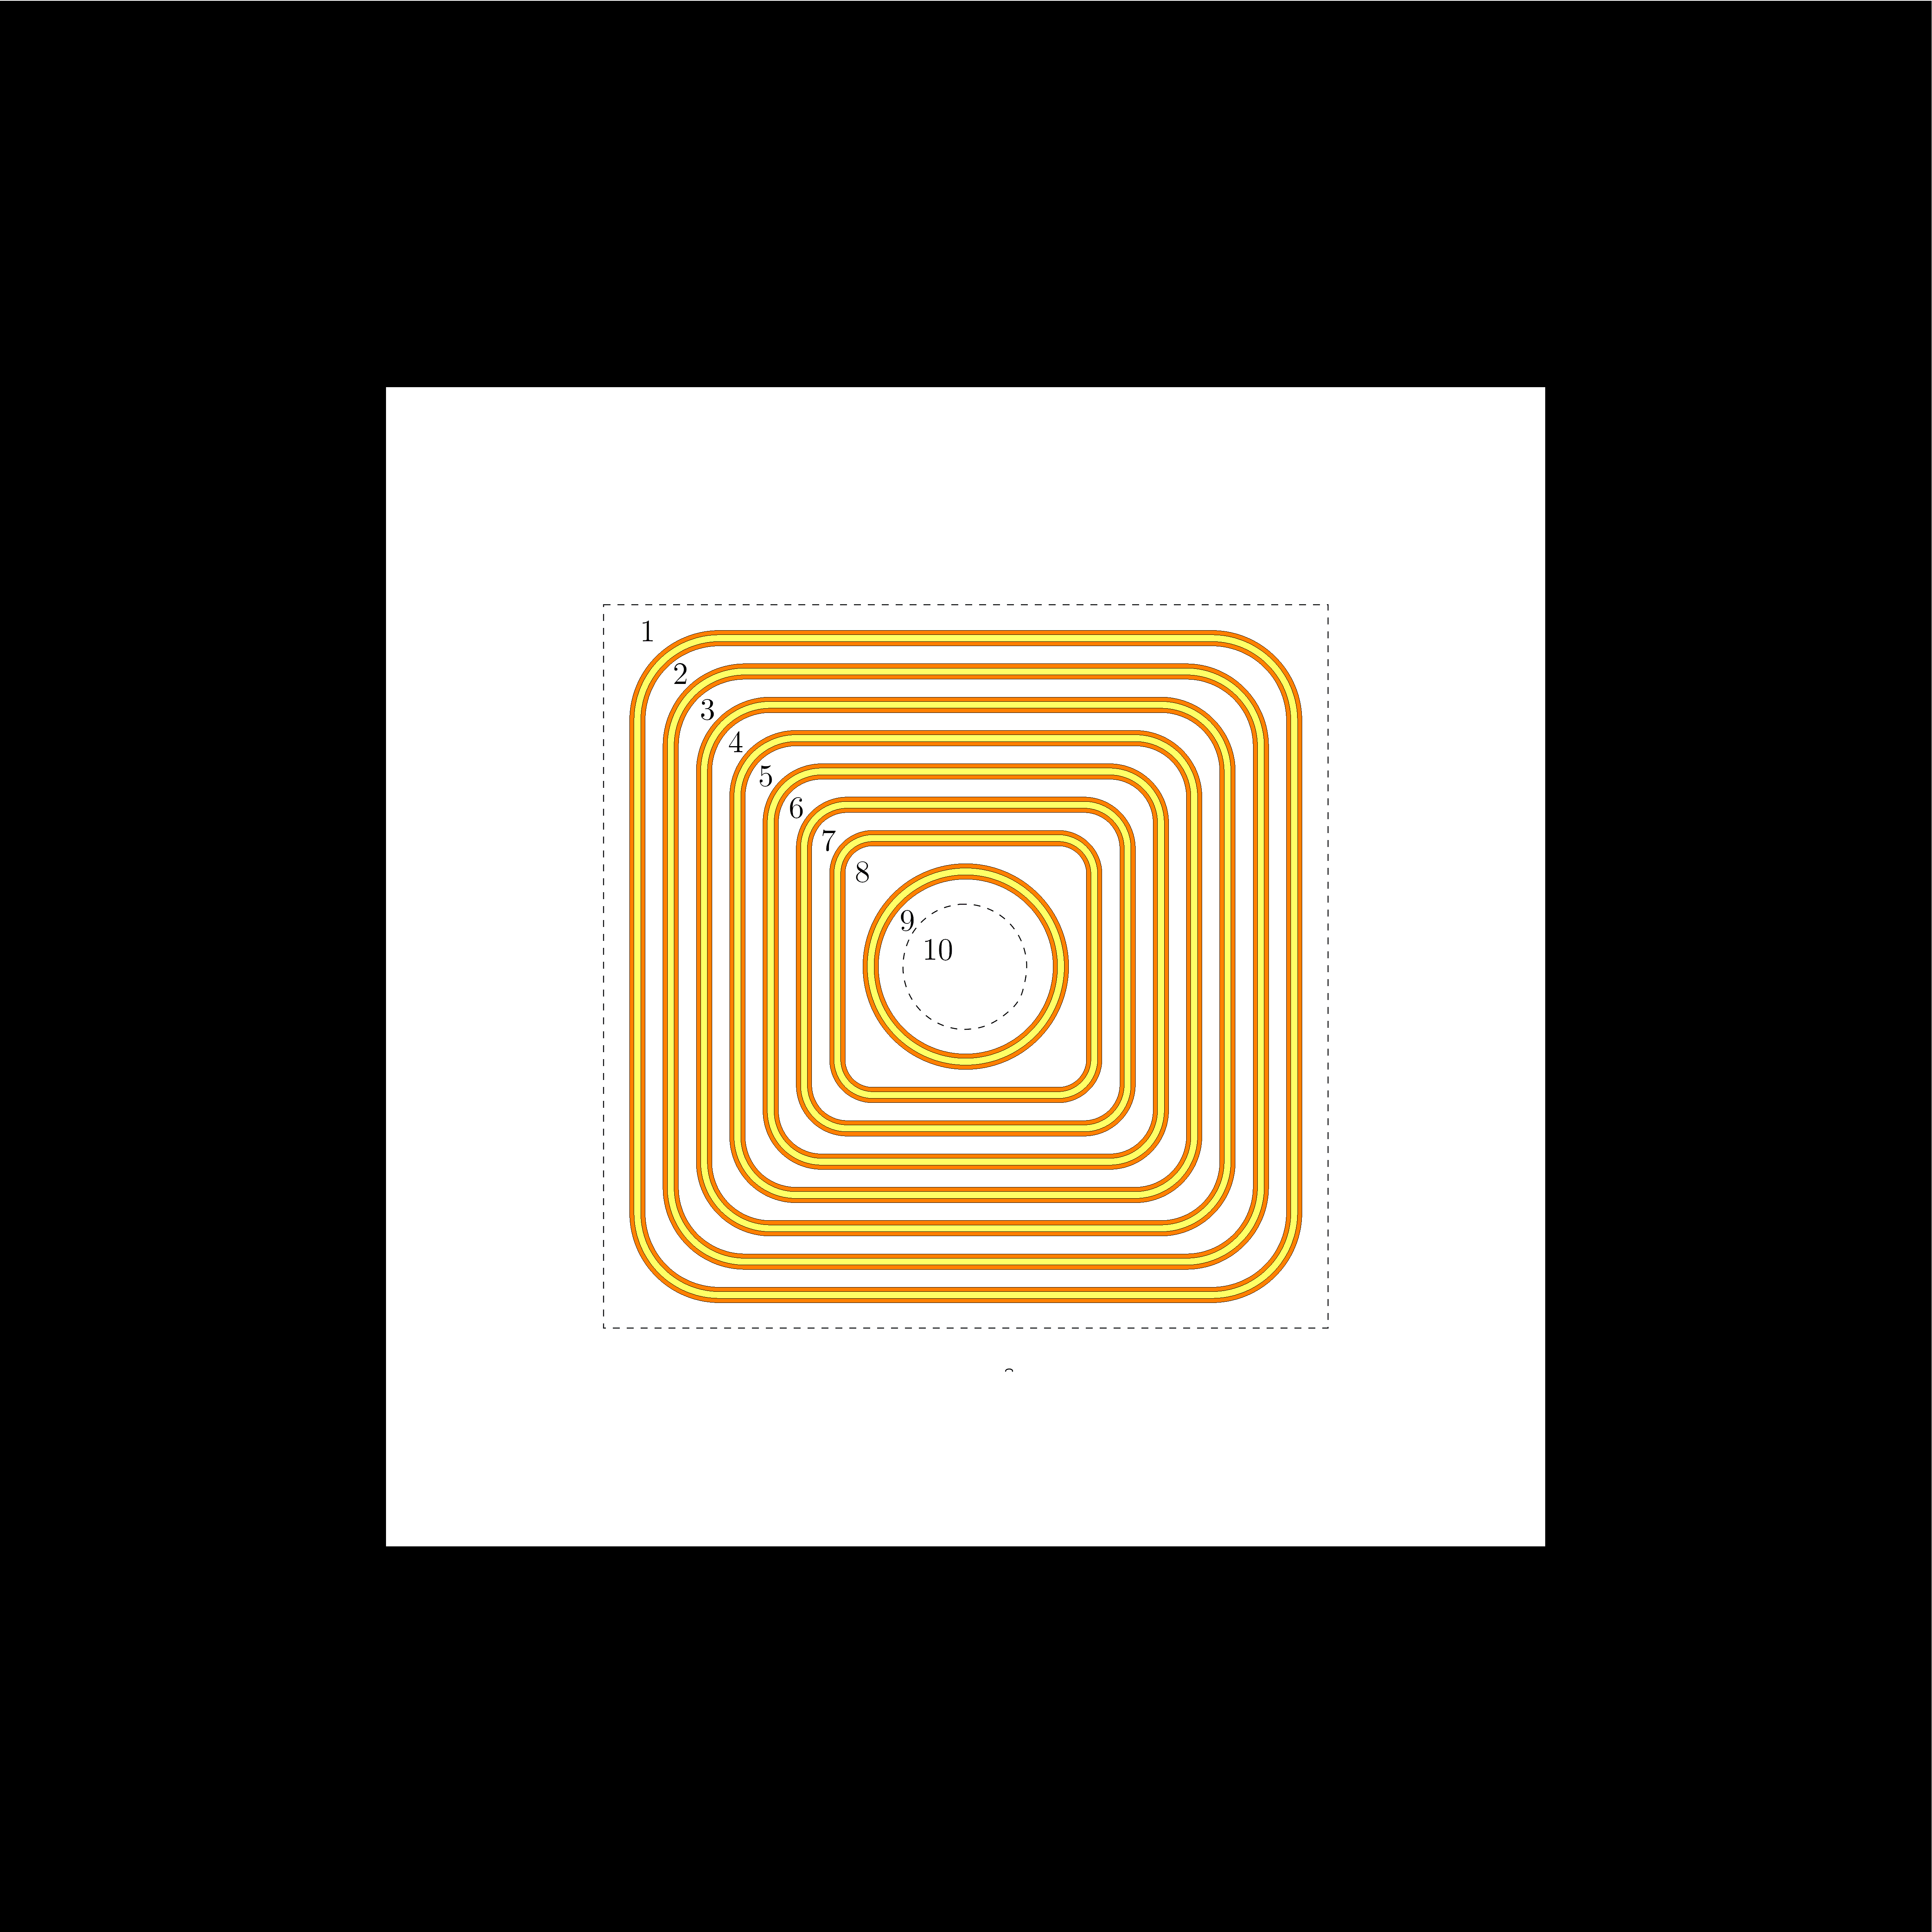
\includegraphics[width=.8\textwidth, trim={40cm 40cm 40cm 40cm},clip]{./04_TH_model_IRT/obrazky/serpent_irt_hor_2.png}
		\caption{Radiální řez palivovým článkem IRT-4M.}
		\label{fig:rad_irt_serpent}
		\vspace{1pt}
		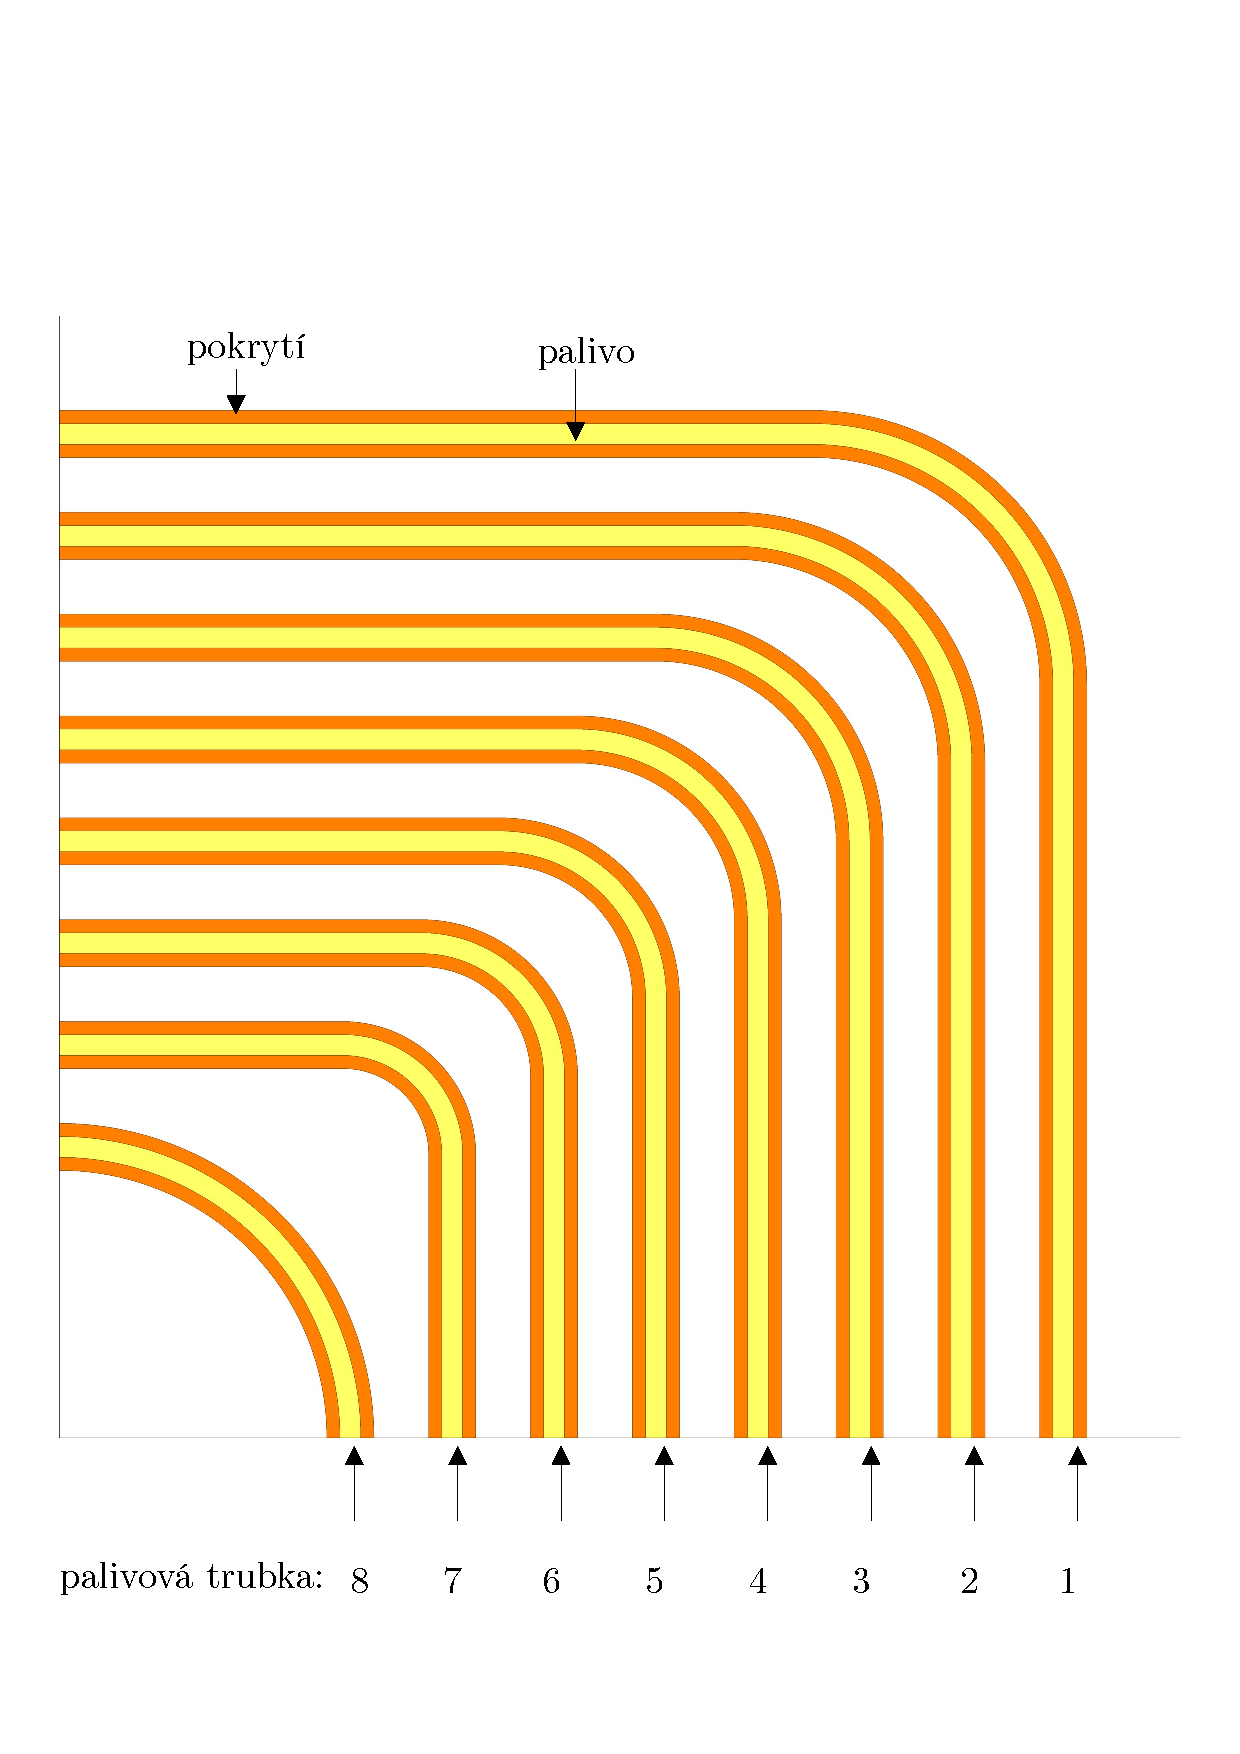
\includegraphics[width=.8\textwidth, trim={1.05cm 0cm 2cm 5.4cm},clip]{./04_TH_model_IRT/obrazky/serpent_irt_detail.pdf}
		\caption{Radiální řez palivovým článkem IRT-4M v detailu.}
		\label{fig:detail_irt_serpent}
	}
	\end{minipage}%
	\begin{minipage}{.5\textwidth}
		\centering
		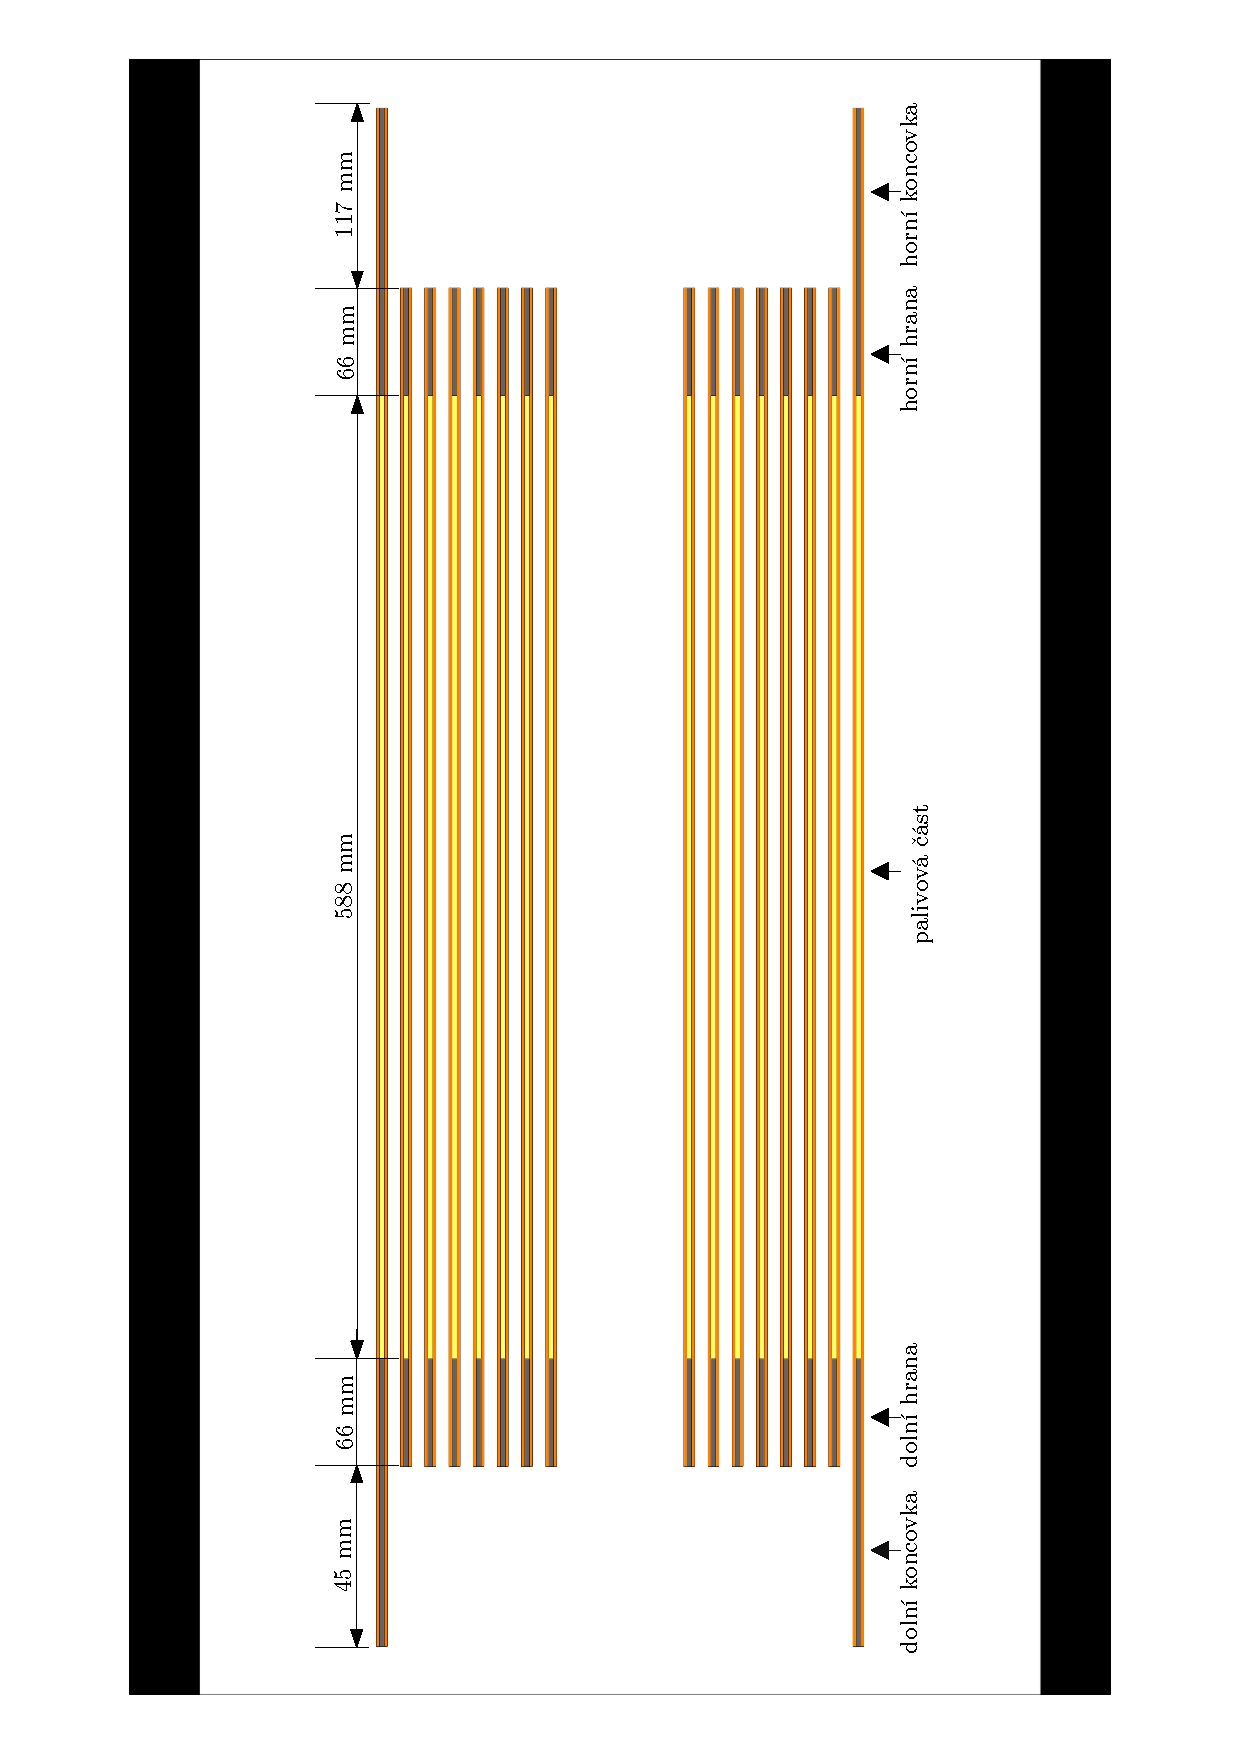
\includegraphics[width=.8\textwidth, trim={5cm 1.5cm 5cm 1.5cm},clip]{./04_TH_model_IRT/obrazky/serpent_irt_ver_2.pdf}
		\caption{Axiální řez palivovým článkem IRT-4M.}
		\label{fig:ax_irt_serpent}
	\end{minipage}
\end{figure}
\begin{figure}
	\centering
	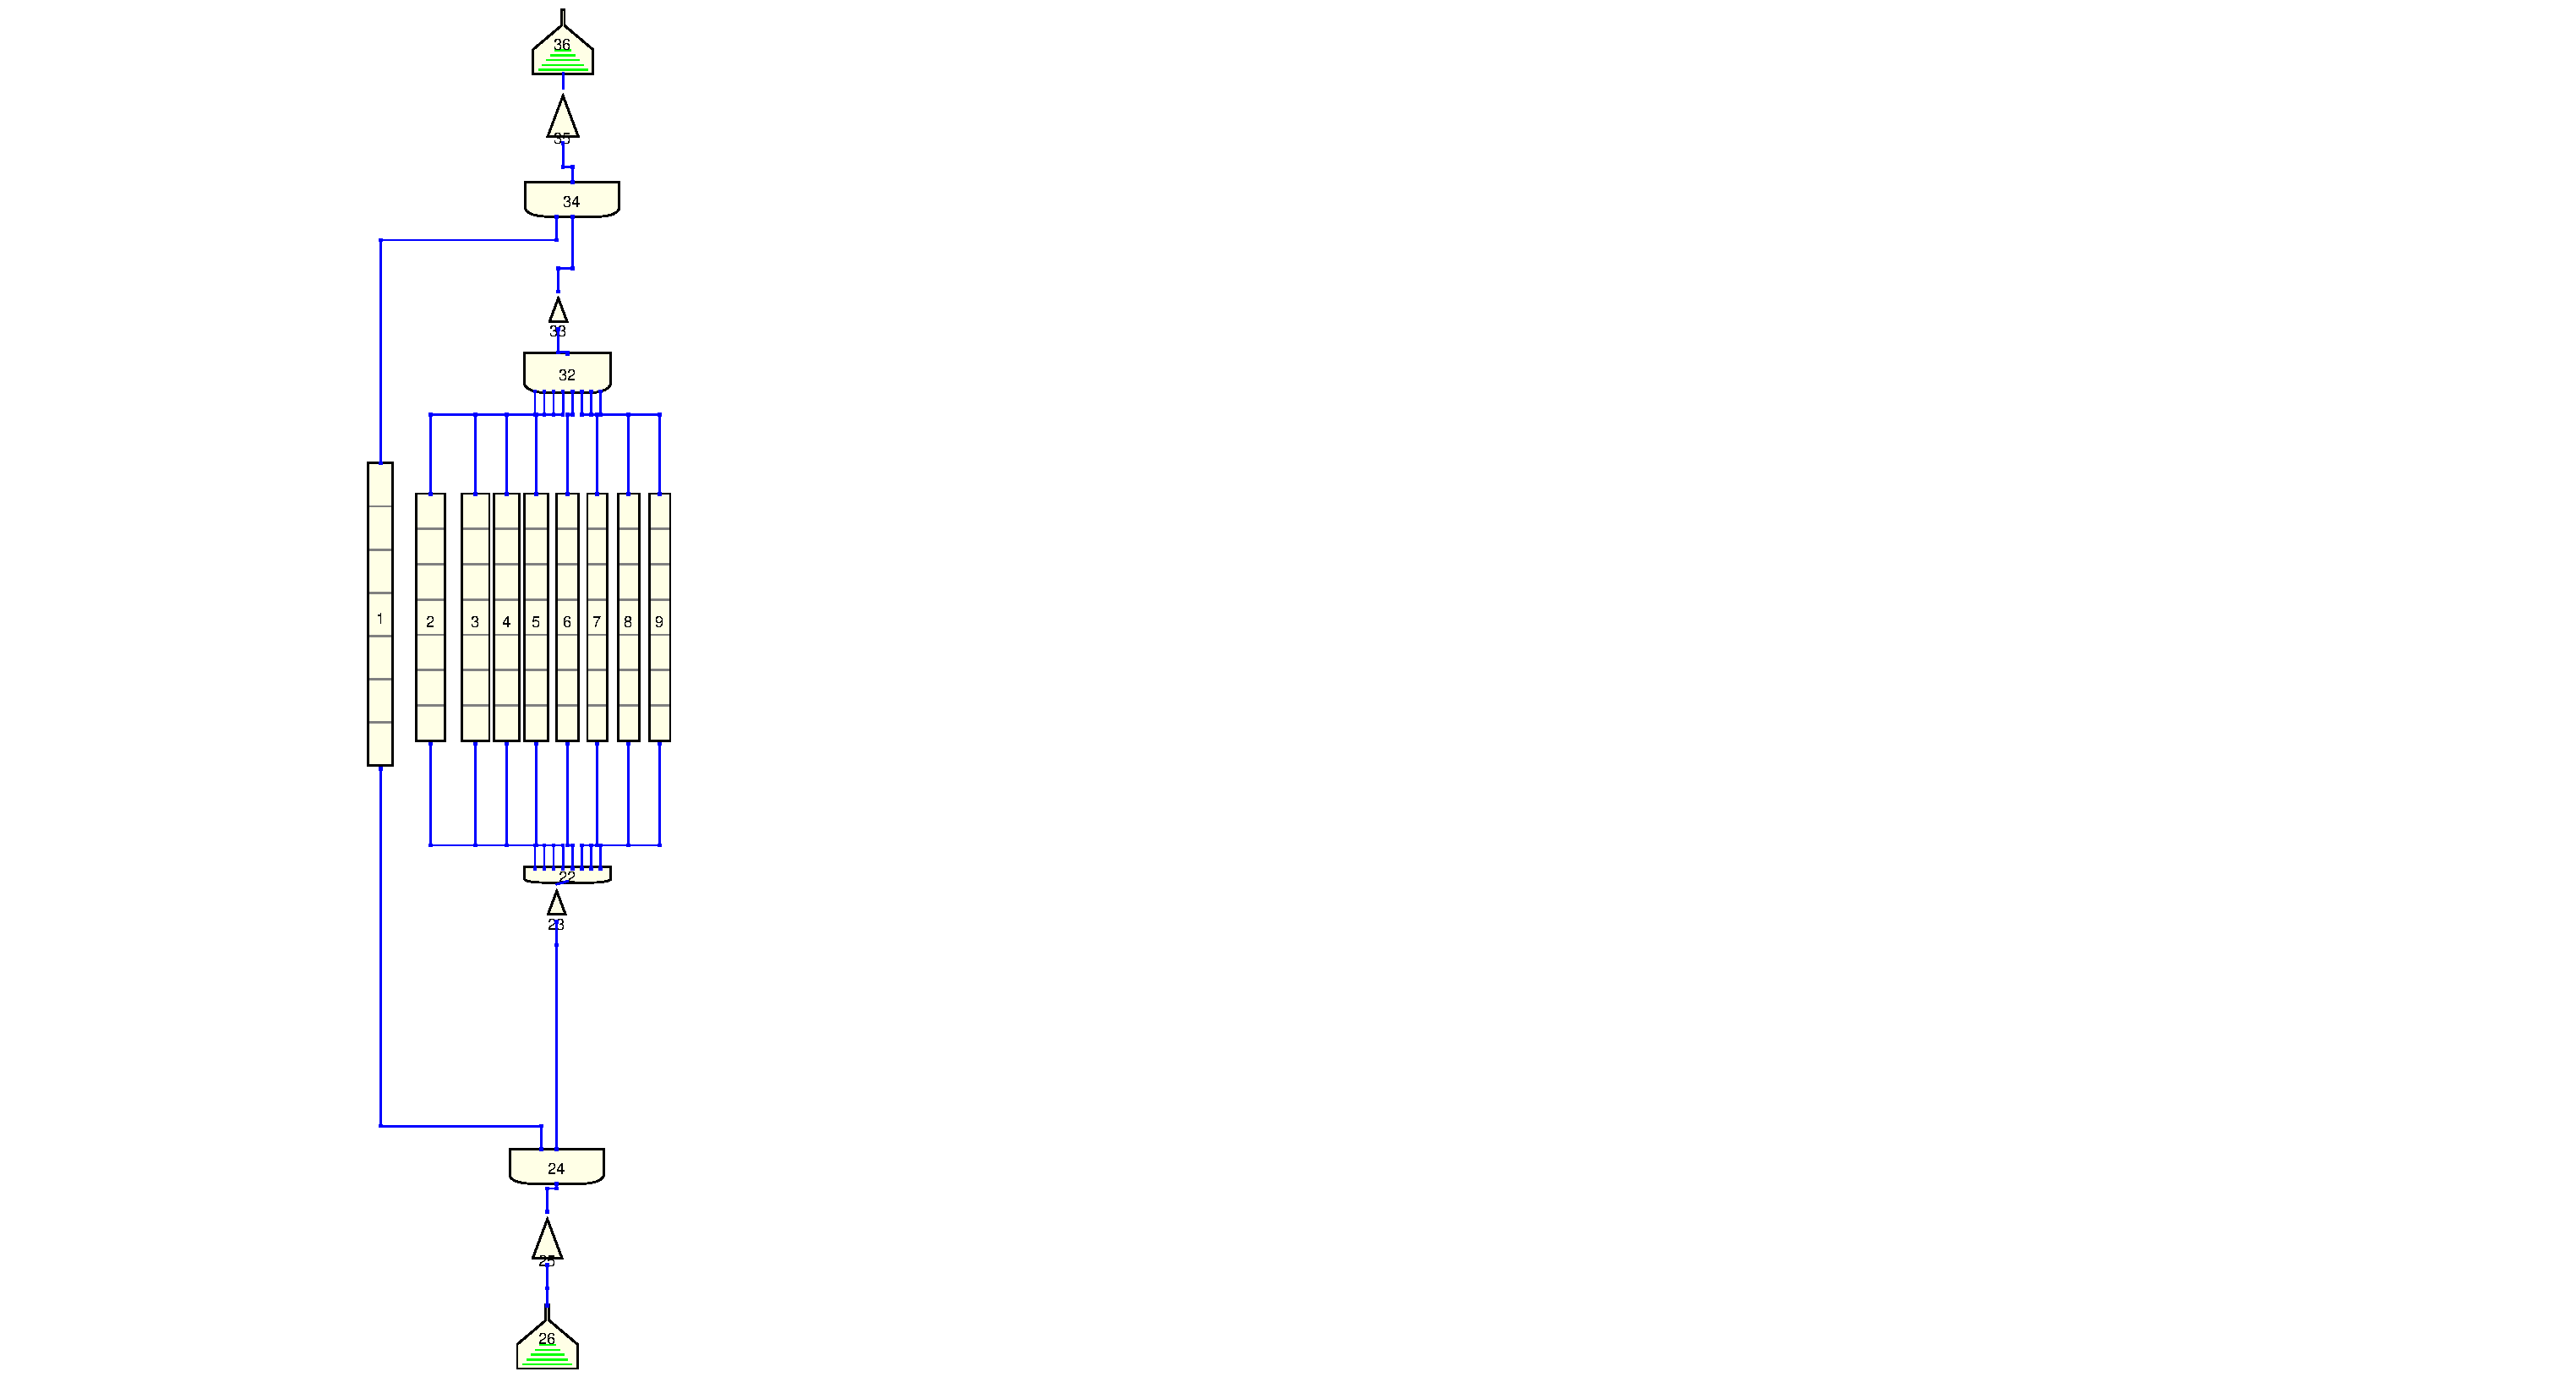
\includegraphics[width=0.6\textwidth, trim={5.5cm 0cm 35cm 0cm},clip]{./04_TH_model_IRT/obrazky/hydraulic_irt_relap.pdf}
	\caption{Hydraulický model palivového článku IRT-4M.}
	\label{fig:irt_hydraulic_relap}
\end{figure}
\newpage
\subsection{Ověření správnosti modelu}
Návrh a ověření modelu vyplývá z \cite{fejt}, kdy výsledné proudění je charakterizováno relativními objemovými průtoky $ G $ (m$ ^3/ $h) skrze průtočné plochy 1-10. Relativní průtoky G$ _i $/G (-) jsou uvedeny v Tab \ref{tab:rel_prutoky}. Celkový objemový průtok 8-trubkovým PČ v závislosti na tlakovém rozdílu vytvořeným odpovídajícím vodním sloupcem je v uveden tab. \ref{tab:celkovy_prutok_vodni_sloupec}. Pro srovnání byly použity výsledky uvedené v \cite{sedlbauer2019} (výsledky jsou označeny jako referenční). 
% Please add the following required packages to your document preamble:
% \usepackage[table,xcdraw]{xcolor}
% If you use beamer only pass "xcolor=table" option, i.e. \documentclass[xcolor=table]{beamer}
\begin{table}[H]
	\centering
	\caption{Relativní objemové průtoky skrze palivový článek (s odpovídajícím vytěsnitelem).}
	\label{tab:rel_prutoky}
	\resizebox{\textwidth}{!}{
		\begin{tabular}{ccccccc}
			\hline
			& \multicolumn{6}{c}{\textbf{G$_i$/G (-)}}   \\ \hline                                      
			Průtočná plocha & \multicolumn{2}{c}{\textbf{8-trubkový PČ}}                             & \multicolumn{2}{l}{\textbf{6-trubkový PČ}}                             & \multicolumn{2}{l}{\textbf{4-trubkový PČ}}                             \\ \hline \hline
			& RELAP5 & Referenční & RELAP5 & Referenční & RELAP5 & Referenční \\ \hline
			1               & 0,122 & 0,114 & 0,145 &0,130 & 0,182 & 0,173 \\
			2               & 0,165                         & 0,151                         & 0,194                         & 0,173                         & 0,243                         & 0,229                         \\
			3               & 0,147                         & 0,148                         & 0,174                         & 0,170                         & 0,218                         & 0,224                         \\
			4               & 0,130                         & 0,135                         & 0,153                         & 0,155                         & 0,192                         & 0,205                         \\
			5               & 0,112                         & 0,112                         & 0,132                         & 0,128                         & 0,166                         & 0,170                         \\
			6               & 0,095                         & 0,111                         & 0,112                         & 0,127                         &                               &                               \\
			7               & 0,077                         & 0,088                         & 0,091                         & 0,117                         &                               &                               \\
			8               & 0,115                         & 0,093                         & 0,000                         & 0,000                         &                               &                               \\
			9               & 0,035                         & 0,040                         &                               &                               &                               &                               \\
			10              & 0,003                         & 0,008                         &                               &                               &                               &                              \\ \hline
		\end{tabular}
	}
	
\end{table}



\begin{table}[H]
	\centering
	\caption{Celkový objemový průtok 8-trubkovým PČ (s vytěsnitelem).}
	\label{tab:celkovy_prutok_vodni_sloupec}
	\begin{tabular}{ccc}
		\hline
		$ \Delta  $p (m) & \multicolumn{2}{c}{\textbf{G} (m$ ^3 $/h)} \\ \hline
		& RELAP5 & Referenční \\ 
		\hline \hline
		2,45 & 22,7 & 25,6 \\
		3 & 27,5 & 28,4 \\
		3,5 & 31,3 & 30,7 \\
		4 & 34,8 & 32,8 \\ \hline
		
	\end{tabular}
	
\end{table}
\begin{table}[H]
	\centering
	\caption{Rozložení rychlostí v kanálech 8-trubkového PČ (s vytěsnitelem).}
	\label{tab:rel_rychlosti}
	\begin{tabular}{ccc}
		\hline
		& \multicolumn{2}{c}{\textbf{w }/ \textbf{w}$_{\text{max}} $} \\ \hline
		Průtočná plocha & RELAP5      & Referenční \\ \hline \hline
		1               & 0,81            & 0,84       \\
		2               & 0,77            & 0,78       \\
		3               & 0,77            & 0,86       \\
		4               & 0,77            & 0,89       \\
		5               & 0,77            & 0,86       \\
		6               & 0,77            & 1,00       \\
		7               & 0,77            & 0,98       \\
		8               & 1,00            & 0,90       \\
		9               & 0,78            & 0,98       \\
		10              & 0,05            & 0,18		\\ \hline      
	\end{tabular}
	
\end{table}
\begin{figure}[H]
	\centering
	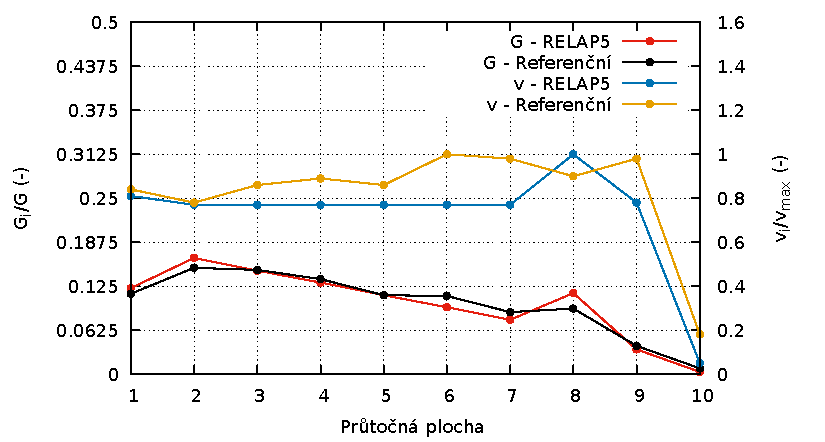
\includegraphics[width=\textwidth]{./04_TH_model_IRT/grafy/rozdeleni_v_g.pdf}
	\caption{Průtok a rychlost v jednotlivých kanálech.}
	\label{fig:rozdeleni_v_g}
\end{figure}
Na Obr. \ref{fig:rozdeleni_v_g} je vykresleno rozdělení relativních průtoků a rychlostí pro 8-trubkový palivový článek s vytěsnitelem. Model vytvořený v RELAP5 dává větší rozdíly v průtocích, rozdělení rychlostí dává naopak rovnoměrnější hodnoty. Odchylky od referenčních hodnot mohou být způsobeny mnoha faktory a naprostá shoda se nedala očekávat. Tyto odchylky ovšem nemají pro další výpočty zásadní vliv a model může být považován za vhodný.

\section{Zjednodušený hydraulický model}
\label{sec:zjednoduseny_hydraulicky_model_irt}
V aktivní zóně reaktoru VR-1 je okolo 16 palivových článků, což dává okolo 160 průtočných kanálů (při uvažování 8-trubkových PČ S vytěsnitelem) pro celý model reaktoru. Pro lepší použitelnost modelu při výpočtech obsahujících externí 3D kinetiku je vhodnější vytvořit zjednodušený model palivového článku se sjednoceným kanálem (viz Obr. \ref{fig:irt_hydraulic_simple_relap}). Při sjednocení kanálů je třeba zachovat celkovou průtočnou plochu a získat adekvátní hydraulický průměr, který zaručí stejný průtok. Prvním odhad hydraulického průměru vychází z rovnice:
\begin{equation}
	d_h = \frac{4S}{o},
	\label{eq:dh}
\end{equation}
kde $S$, resp. $o$ je celková průtočná plocha, resp. celkový omočený obvod palivového článku. Následně byl průměr iterován pro získání průtoku z komplexního modelu viz Obr. \ref{fig:iterated_dh}. Zjednodušený hydraulický model PČ uvedený na Obr. \ref{fig:irt_hydraulic_simple_relap} je v následujících kapitolách využit k vytvoření termohydraulického \uv{jednotkového} modelu (viz sekce \ref{sec:termohydraulicky_model}), který představuje PČ v modelu reaktoru VR-1.

\begin{figure}
	\centering
	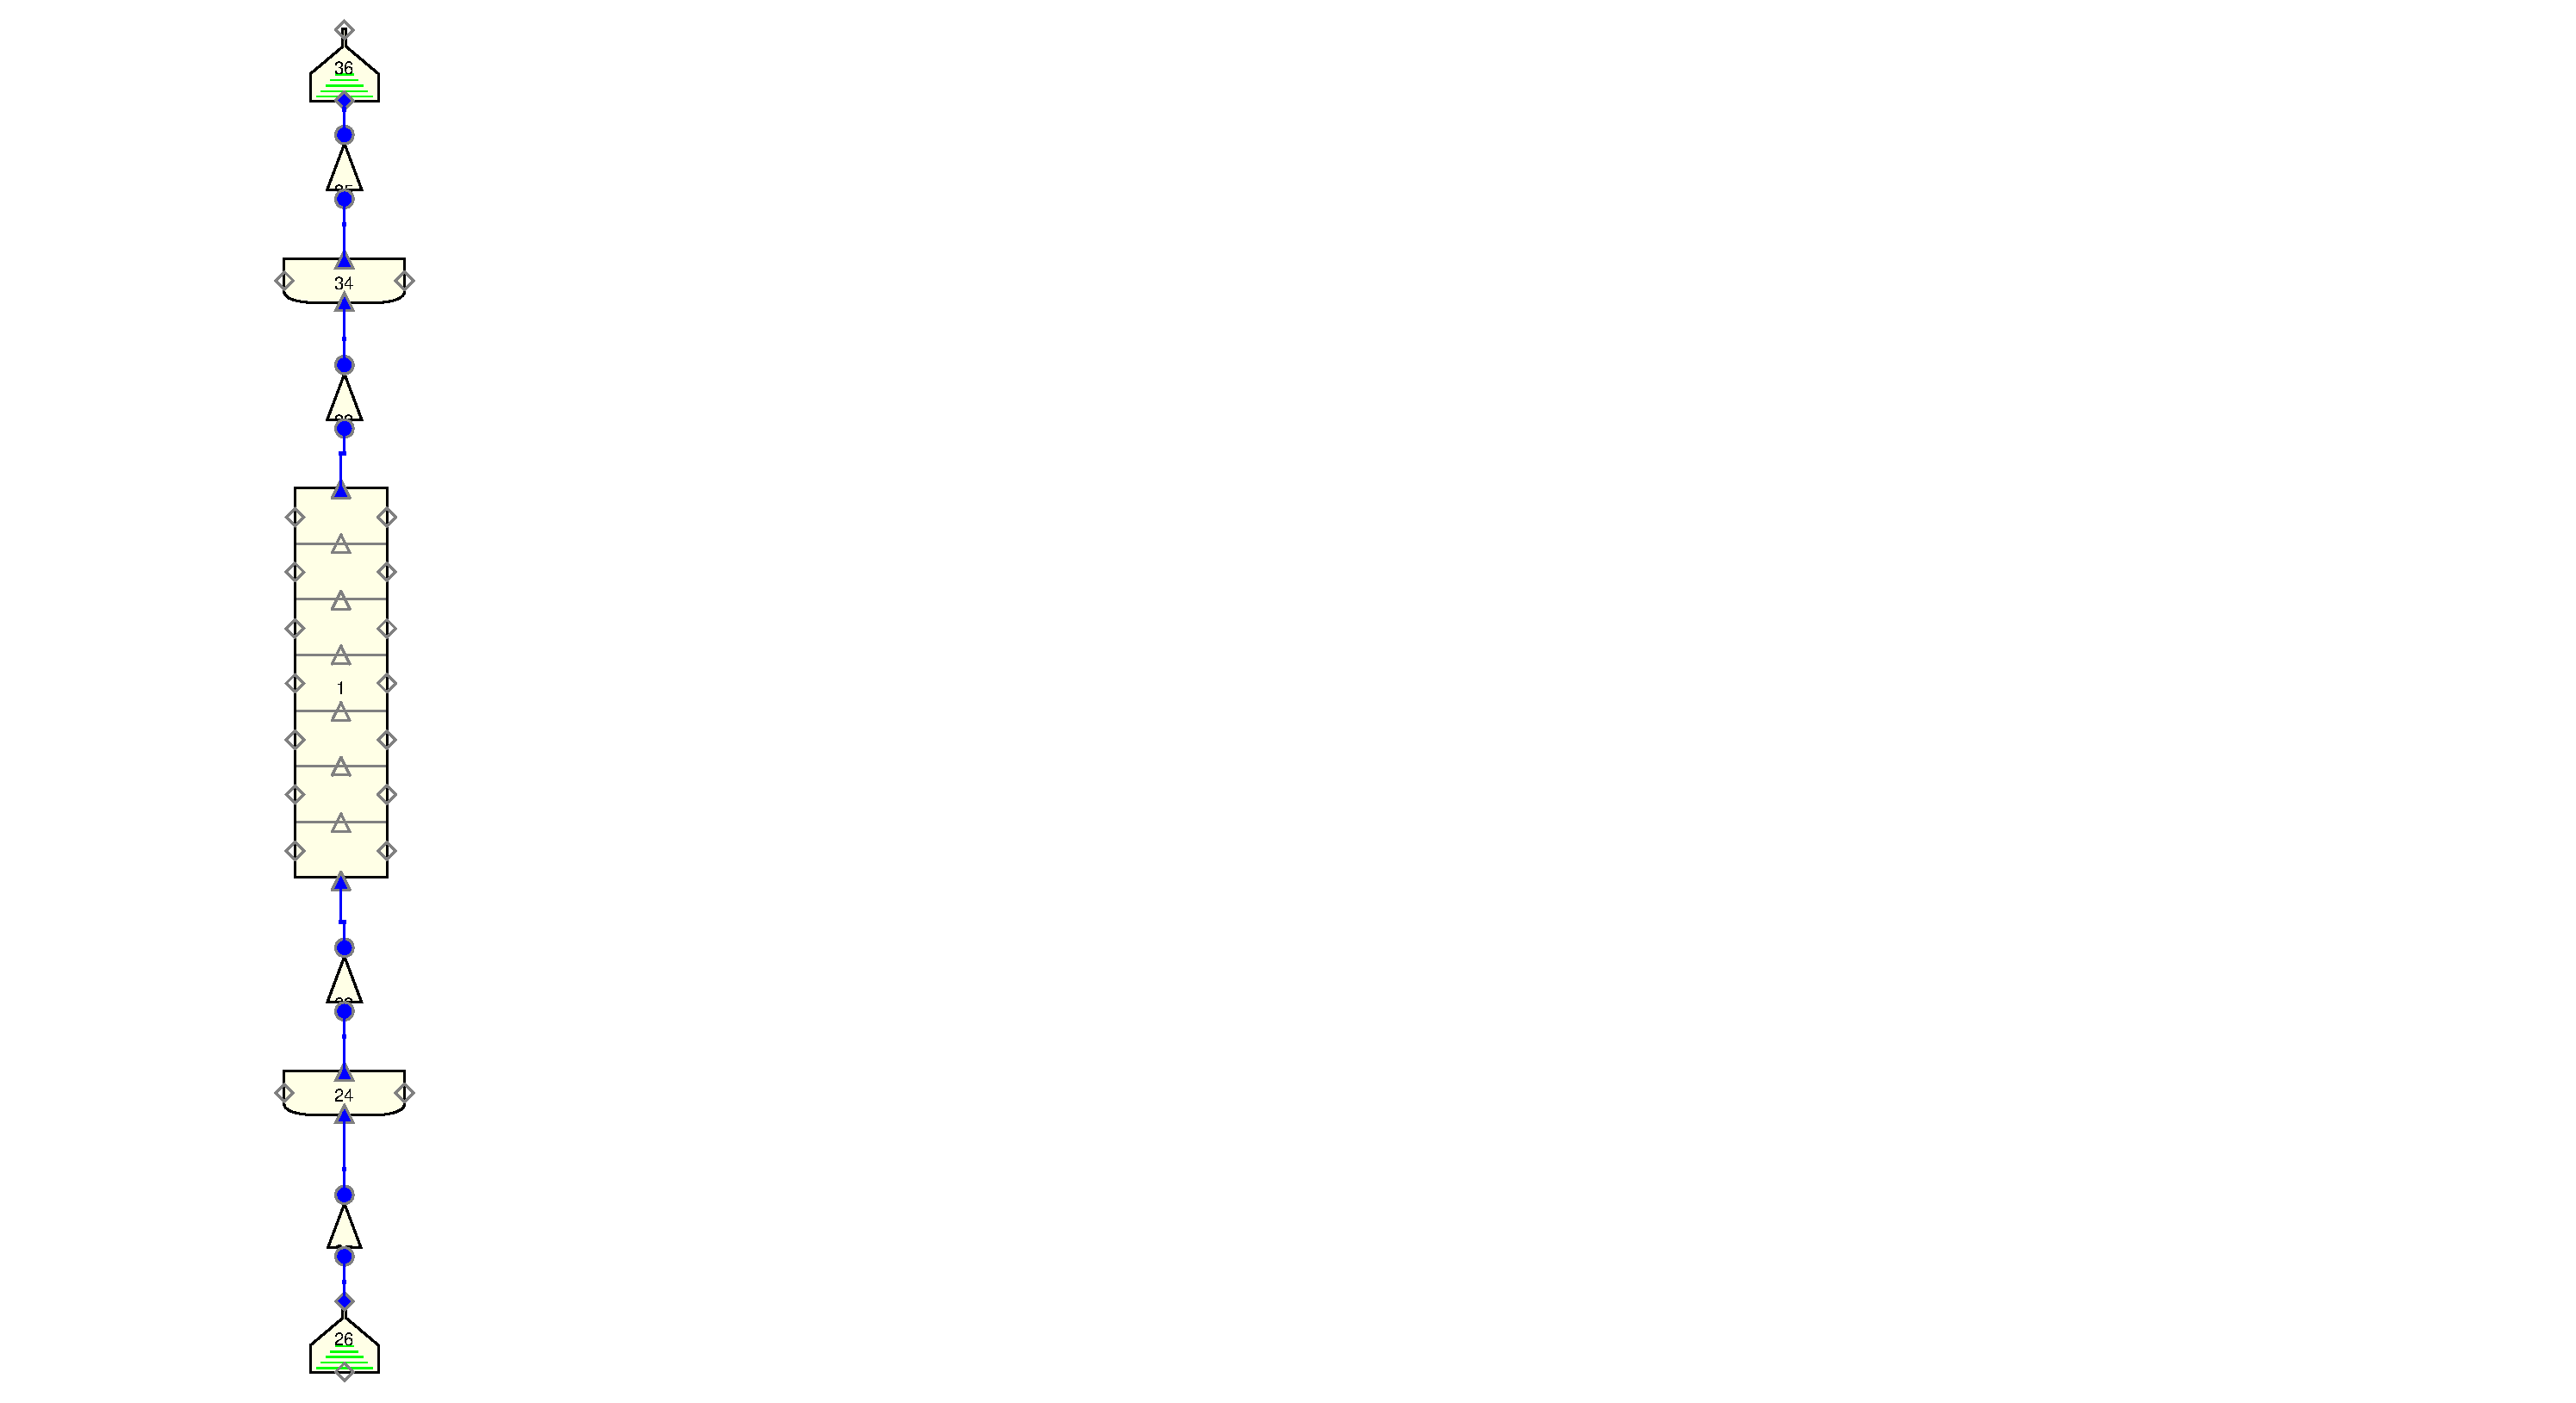
\includegraphics[width=0.6\textwidth, trim={0cm 0cm 39cm 0cm},clip]{./04_TH_model_IRT/obrazky/hydraulic_irt_simple_relap.pdf}
	\caption{Zjednodušený hydraulický model palivového článku IRT-4M.}
	\label{fig:irt_hydraulic_simple_relap}
\end{figure}
\subsection{Ověření správnosti modelu}
Závislost průtoku na hydraulickém průměru zjednodušeného modelu je vykreslena na Obr. \ref{fig:iterated_dh}. Rozdíl tlaku $\Delta p$ odpovídá 4 metrům vodního sloupce.
\begin{figure}[H]
	\centering
	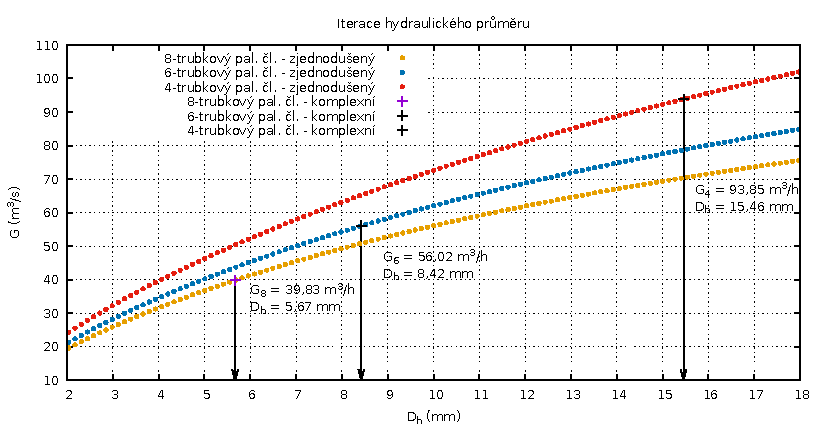
\includegraphics[width=\textwidth]{./04_TH_model_IRT/grafy/extrapolace_dh.pdf}
	\caption{Závislost průtoku skrz PČ (bez vytěsnitele) na hydraulickém průměru.}
	\label{fig:iterated_dh}
\end{figure}
V Tab. \ref{tab:prutoky_it_srovnani} jsou uvedeny získané hydraulické průměry s odpovídajícím průtokem.
\begin{table}[H]
	\centering
	\caption{Průtok v komplexním a zjednodušeném modelu PČ (bez vytěsnitele) pro různé hydraulické průměry. }
	\label{tab:prutoky_it_srovnani}
	\begin{tabular}{cccc}
		\hline
		& \textbf{G} (m$^3$/h) - komplex. & \textbf{G} (m$^3$/h) - rovnice \ref{eq:dh} & $d_h$ (mm) - rovnice \ref{eq:dh} \\
		\hline \hline
		4-trubkový PČ & 93,85  & 65,70 & 8,52 \\
		6-trubkový PČ & 56,02  & 43,73 & 5,68 \\
		8-trubkový PČ & 39,83  & 34,68 & 4,59 \\
		\hline
		&&&\\
		&&&\\
		\hline 
		& \textbf{G} (m$^3$/h) - komplex.& \textbf{G} (m$^3$/h) - iterace & $d_h$ (mm) - iterace  \\
		\hline \hline
		4-trubkový PČ & 93,85  & 93,85 & 15,46 \\
		6-trubkový PČ & 56,02  & 56,02 & 8,42 \\
		8-trubkový PČ & 39,83  & 39,84 & 5,67 \\
		\hline 

	\end{tabular}

\end{table}	
Cílem sekce \ref{sec:hydraulicky_model_irt} a \ref{sec:zjednoduseny_hydraulicky_model_irt} bylo vytvoření hydraulického modelu, který je použitelný pro model reaktoru VR-1. Nejzásadnějším krokem popsaným v těchto kapitolách je sjednocení průtočných kanálů, které by mělo zajistit vhodnou strukturu pro následující výpočty. Iterací hydraulického průměru bylo dosaženo identického průtoku a je možné považovat zjednodušený hydraulický model za dostatečný.
\newpage

\section{Termohydraulický model PČ IRT-4M}
\label{sec:termohydraulicky_model}
V předchozí sekci byl prezentován model PČ, ve kterém docházelo k nucenému proudění určeného rozdílem v tlaku na okrajích rozhraní. Tyto okrajové podmínky byly zajištěny párem TDV. Problém je, že školní reaktor VR-1 je charakteristický odvodem tepla za pomocí přirozeného proudění a je nutné vytvořit model, který tuto skutečnost bude respektovat a co nejlépe popisovat. Z \cite{fejt} vyplývá, že kromě vhodně zvolených komponent je třeba také zvolit sledované fyzikální veličiny pro co nejvíce přesnou interpretaci a srovnání výsledků.

Při srovnání Obr. \ref{fig:irt_hydraulic_relap} a \ref{fig:irt_nat_conv_komplex} lze vidět, že pár TDV byl zaměněn za smyčku složenou z trubek a spojovacích komponent, která představuje obtok okolo PČ. Výška vertikálního kruhové trubky obtoku byla nastavena na 3,555 m a její průměr na 2,3 m, což zhruba odpovídá geometrii reaktorové nádoby. Dále byl ke komponentě 53 připojena TDV simulující otevřenou vodní hladinu při atmosférickém tlaku (p = 101,325 kPa, T = 293 K). V případě komplexního, resp. zjednodušeného modelu byla pro samotný PČ převzata již vytvořená geometrie viz \ref{fig:irt_hydraulic_relap}, resp. \ref{fig:irt_hydraulic_simple_relap}, přičemž konstrukce obtoku zůstává pro obě dvě varianty modelu stejná.

Hlavním problémem při zadávání zdrojů tepla bylo vystihnutí správné geometrie. Jelikož průřez trubkou PČ IRT-4M odpovídá čtverci s kulatými rohy (viz Obr. \ref{fig:rad_irt_serpent}) a geometrie zdrojů tepla (HS) v RELAP5 je značně omezená, musely být jednotlivé trubky napodobeny válcovou geometrií s vnějším a vnitřním průměrem. Tyto parametry byly získány z podmínek na identický objem, teplosměnnou plochu a tloušťku trubek viz \cite{fejt}. Rozměry jednotlivých HS komponent jsou uvedeny v tabulce \ref{tab:equivalent_hs}. Při přechodu z komplexního na zjednodušený model je třeba ověřit zachování fyzikálních veličin \cite{fejt}: 
\begin{itemize}
	\item velikost průtoku skrze PČ vlivem přirozené konvekce,
	\item výstupních teplot,
	\item výskyt varu.
\end{itemize}
Pro ohřev vody v PČ můžeme předpokládat následující zjednodušený vztah:
\begin{equation}
	\Delta T_{cool} = \frac{Q}{\rho \text{ G } c_p } = \frac{Q}{\rho \text{ w } A \,c_p },
\end{equation}
kde Q (W) je tepelný výkon, $\rho$ (kg/m$^3$) je hustota, $c_p$ (J/kg$\cdot$K) měrná tepelná kapacita a A (m$^2$) je průtočná plocha. Pro termohydraulický model bude uvažováno rovnoměrné rozložení výkonu  a rozložení výkonu vycházející z programu Serpent2. Jelikož je celkový výkon pro obě rozdělení totožný, je očekávatelné, že i celkový průtok bude velice podobný. Největší rozdíly se dají očekávat v rozdělení teplot a tudíž i možném výskytu varu.

\begin{table}[H]
	\centering
	\caption{Rozměry ekvivalentních HS pro PČ IRT-4M a jejich napojení na jednotlivé trubky (viz Obr. \ref{fig:irt_nat_conv_komplex} a \ref{fig:irt_nat_conv_jedno}). }
	\label{tab:equivalent_hs}
	\begin{tabular}{ccccccc}
		\hline
		HS &  &  & \multicolumn{2}{c}{Komplexní model} & \multicolumn{2}{c}{Zjednodušený model} \\
		 & $ r_i $ (mm)& $ r_o $ (mm) & $V_i$ & $V_o$ & $V_i$ & $V_o$ \\
		 \hline
		 \hline
		
		1 & 40,17 & 41,77 & 22 & 21 & 11 & 11 \\
		2 & 35,99 & 37,59 & 23 & 22 & 11 & 11 \\
		3 & 31,82 & 33,42 & 24 & 23 & 11 & 11 \\
		4 & 27,65 & 29,25 & 25 & 24 & 11 & 11 \\
		5 & 23,47 & 25,07 & 26 & 25 & 11 & 11 \\
		6 & 19,30 & 20,90 & 27 & 26 & 11 & 11 \\
		7 & 15,12 & 16,72 & 28 & 27 & 11 & 11 \\
		8 & 9,05  & 10,65 & 29 & 28 & 11 & 11  \\
		
		\hline
	\end{tabular}
\end{table}

\begin{figure}[H]
	\centering
	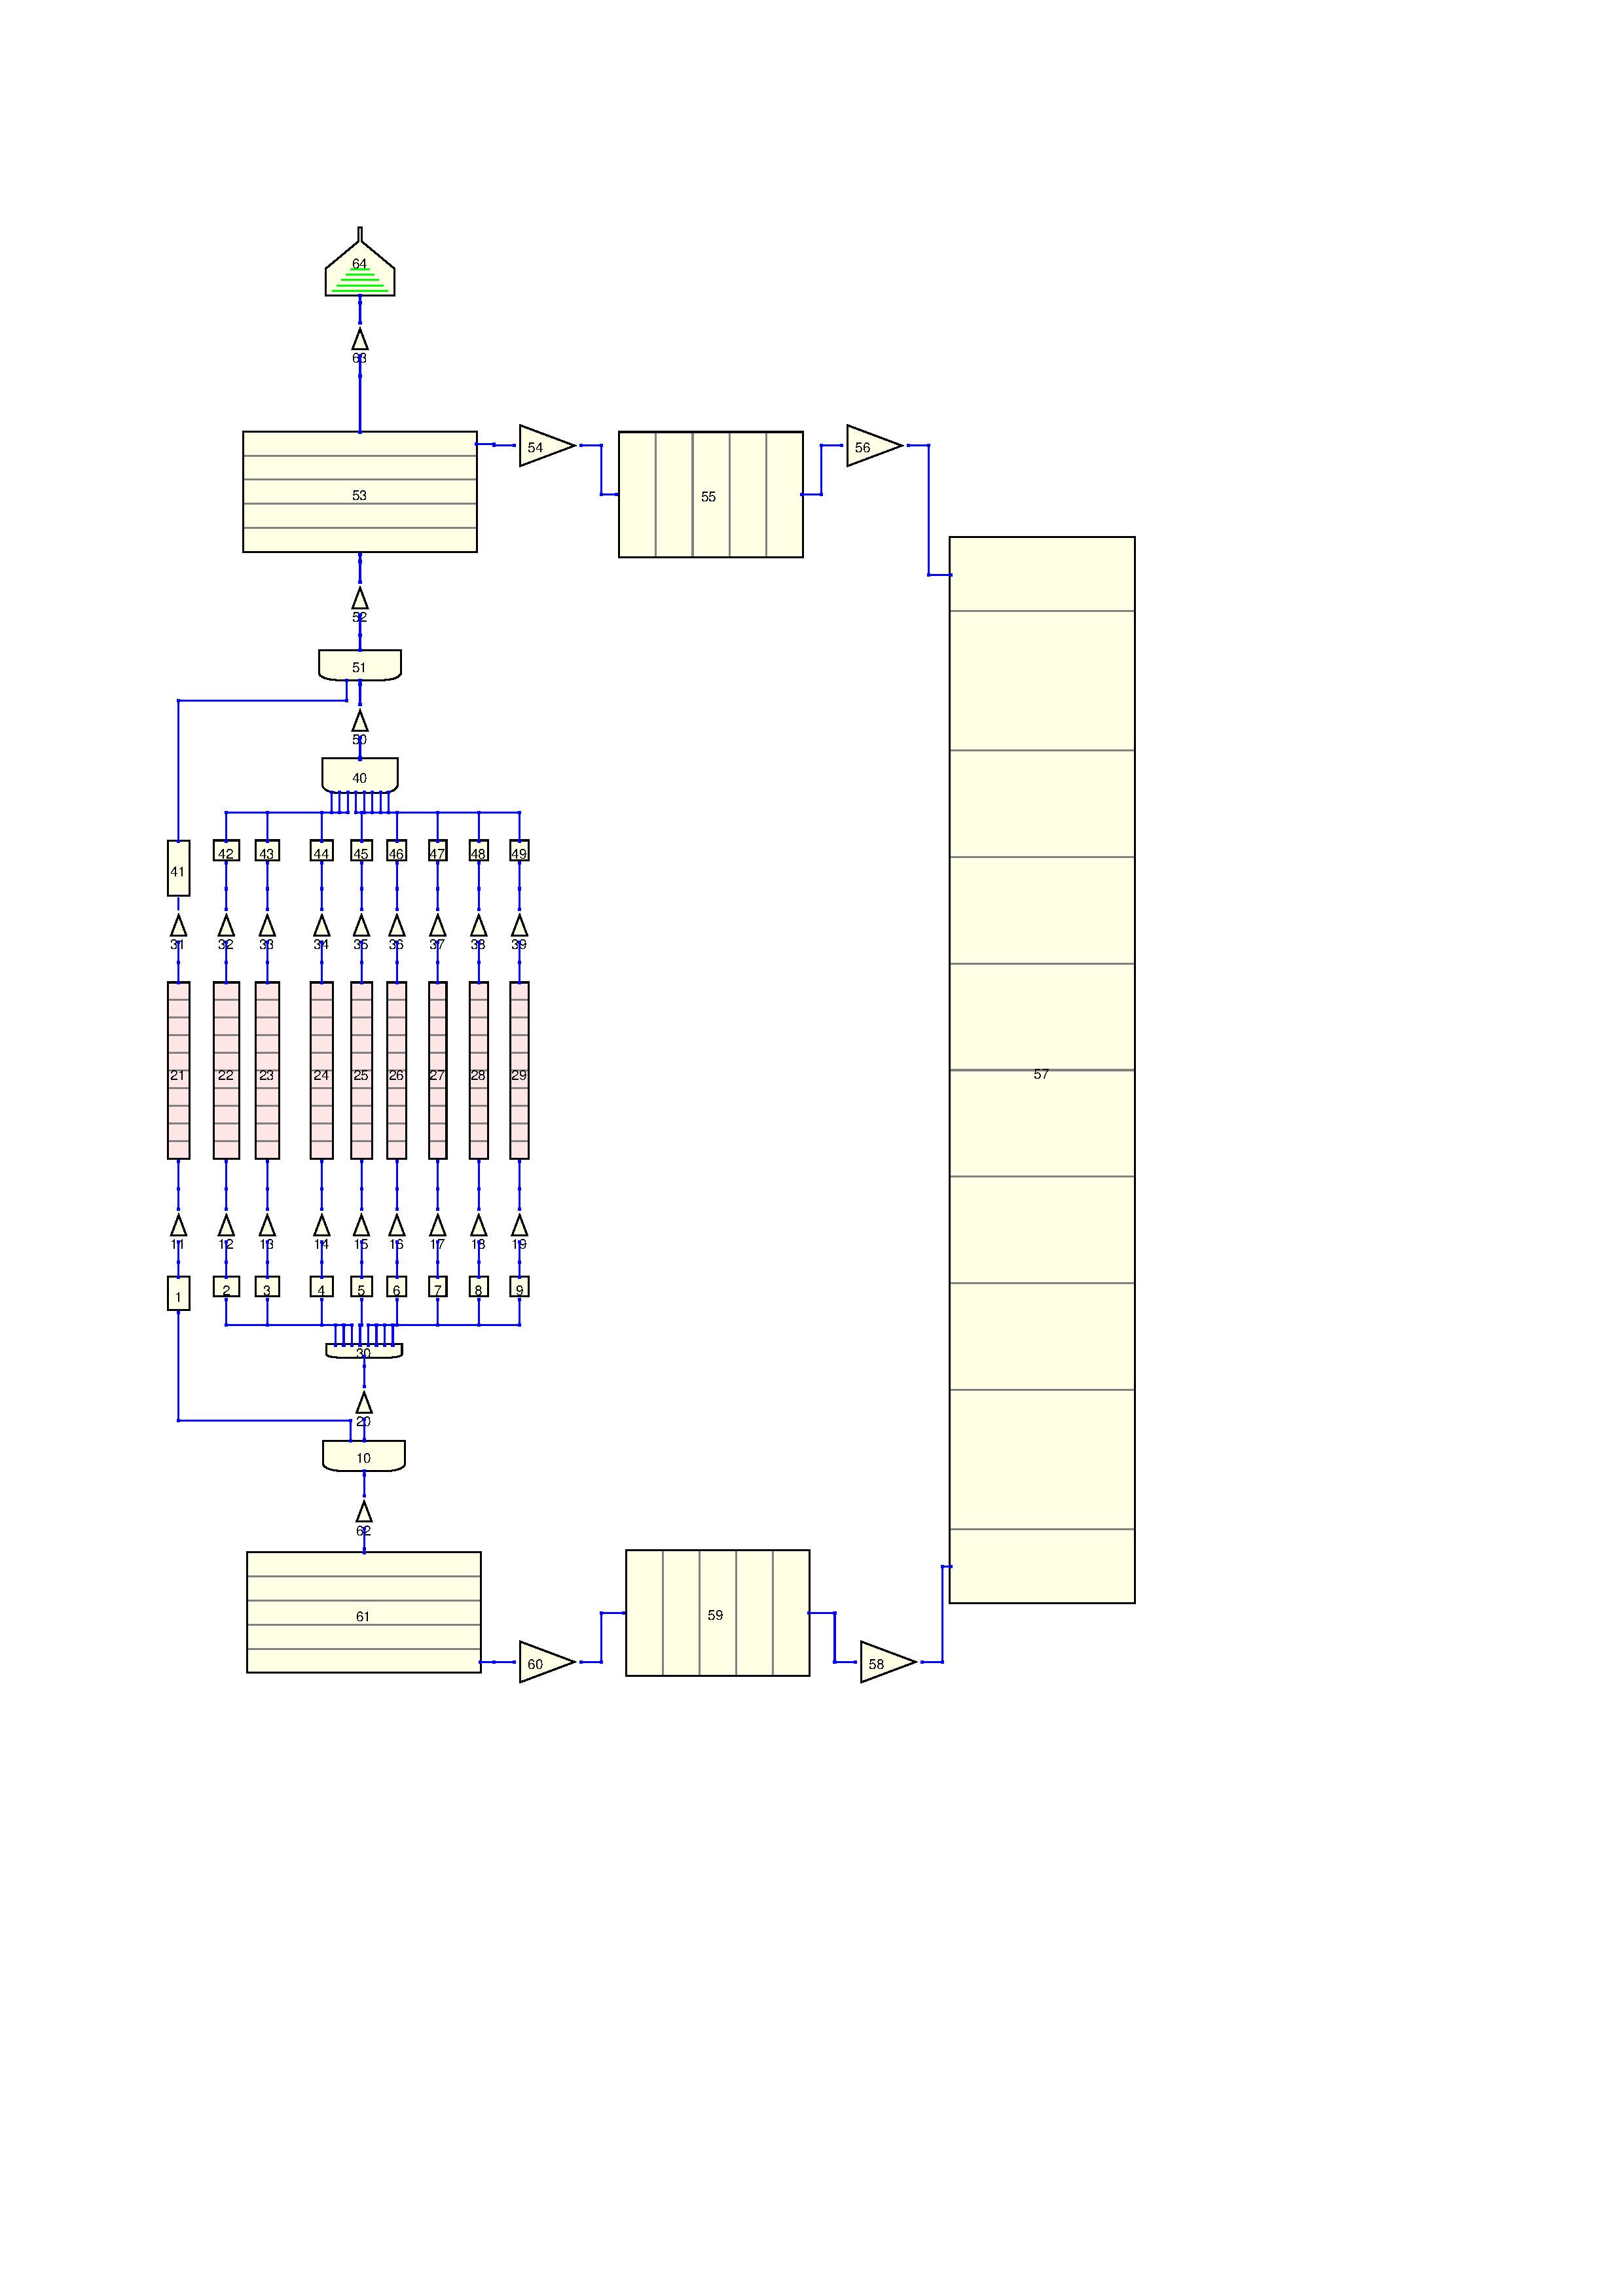
\includegraphics[width=\textwidth, trim={4cm 15cm 12cm 6cm}, clip]{./07_prilohy/prehled_modelu/t8bk.pdf}
	\caption{Termohydraulický komplexní model 8-trubkového PČ IRT-4M bez vytěsnitele (Pro lepší vizualizaci byly měřítka komponent 53 až 62 změněna).}
	\label{fig:irt_nat_conv_komplex}
\end{figure} 
\begin{figure}[H]
	\centering
	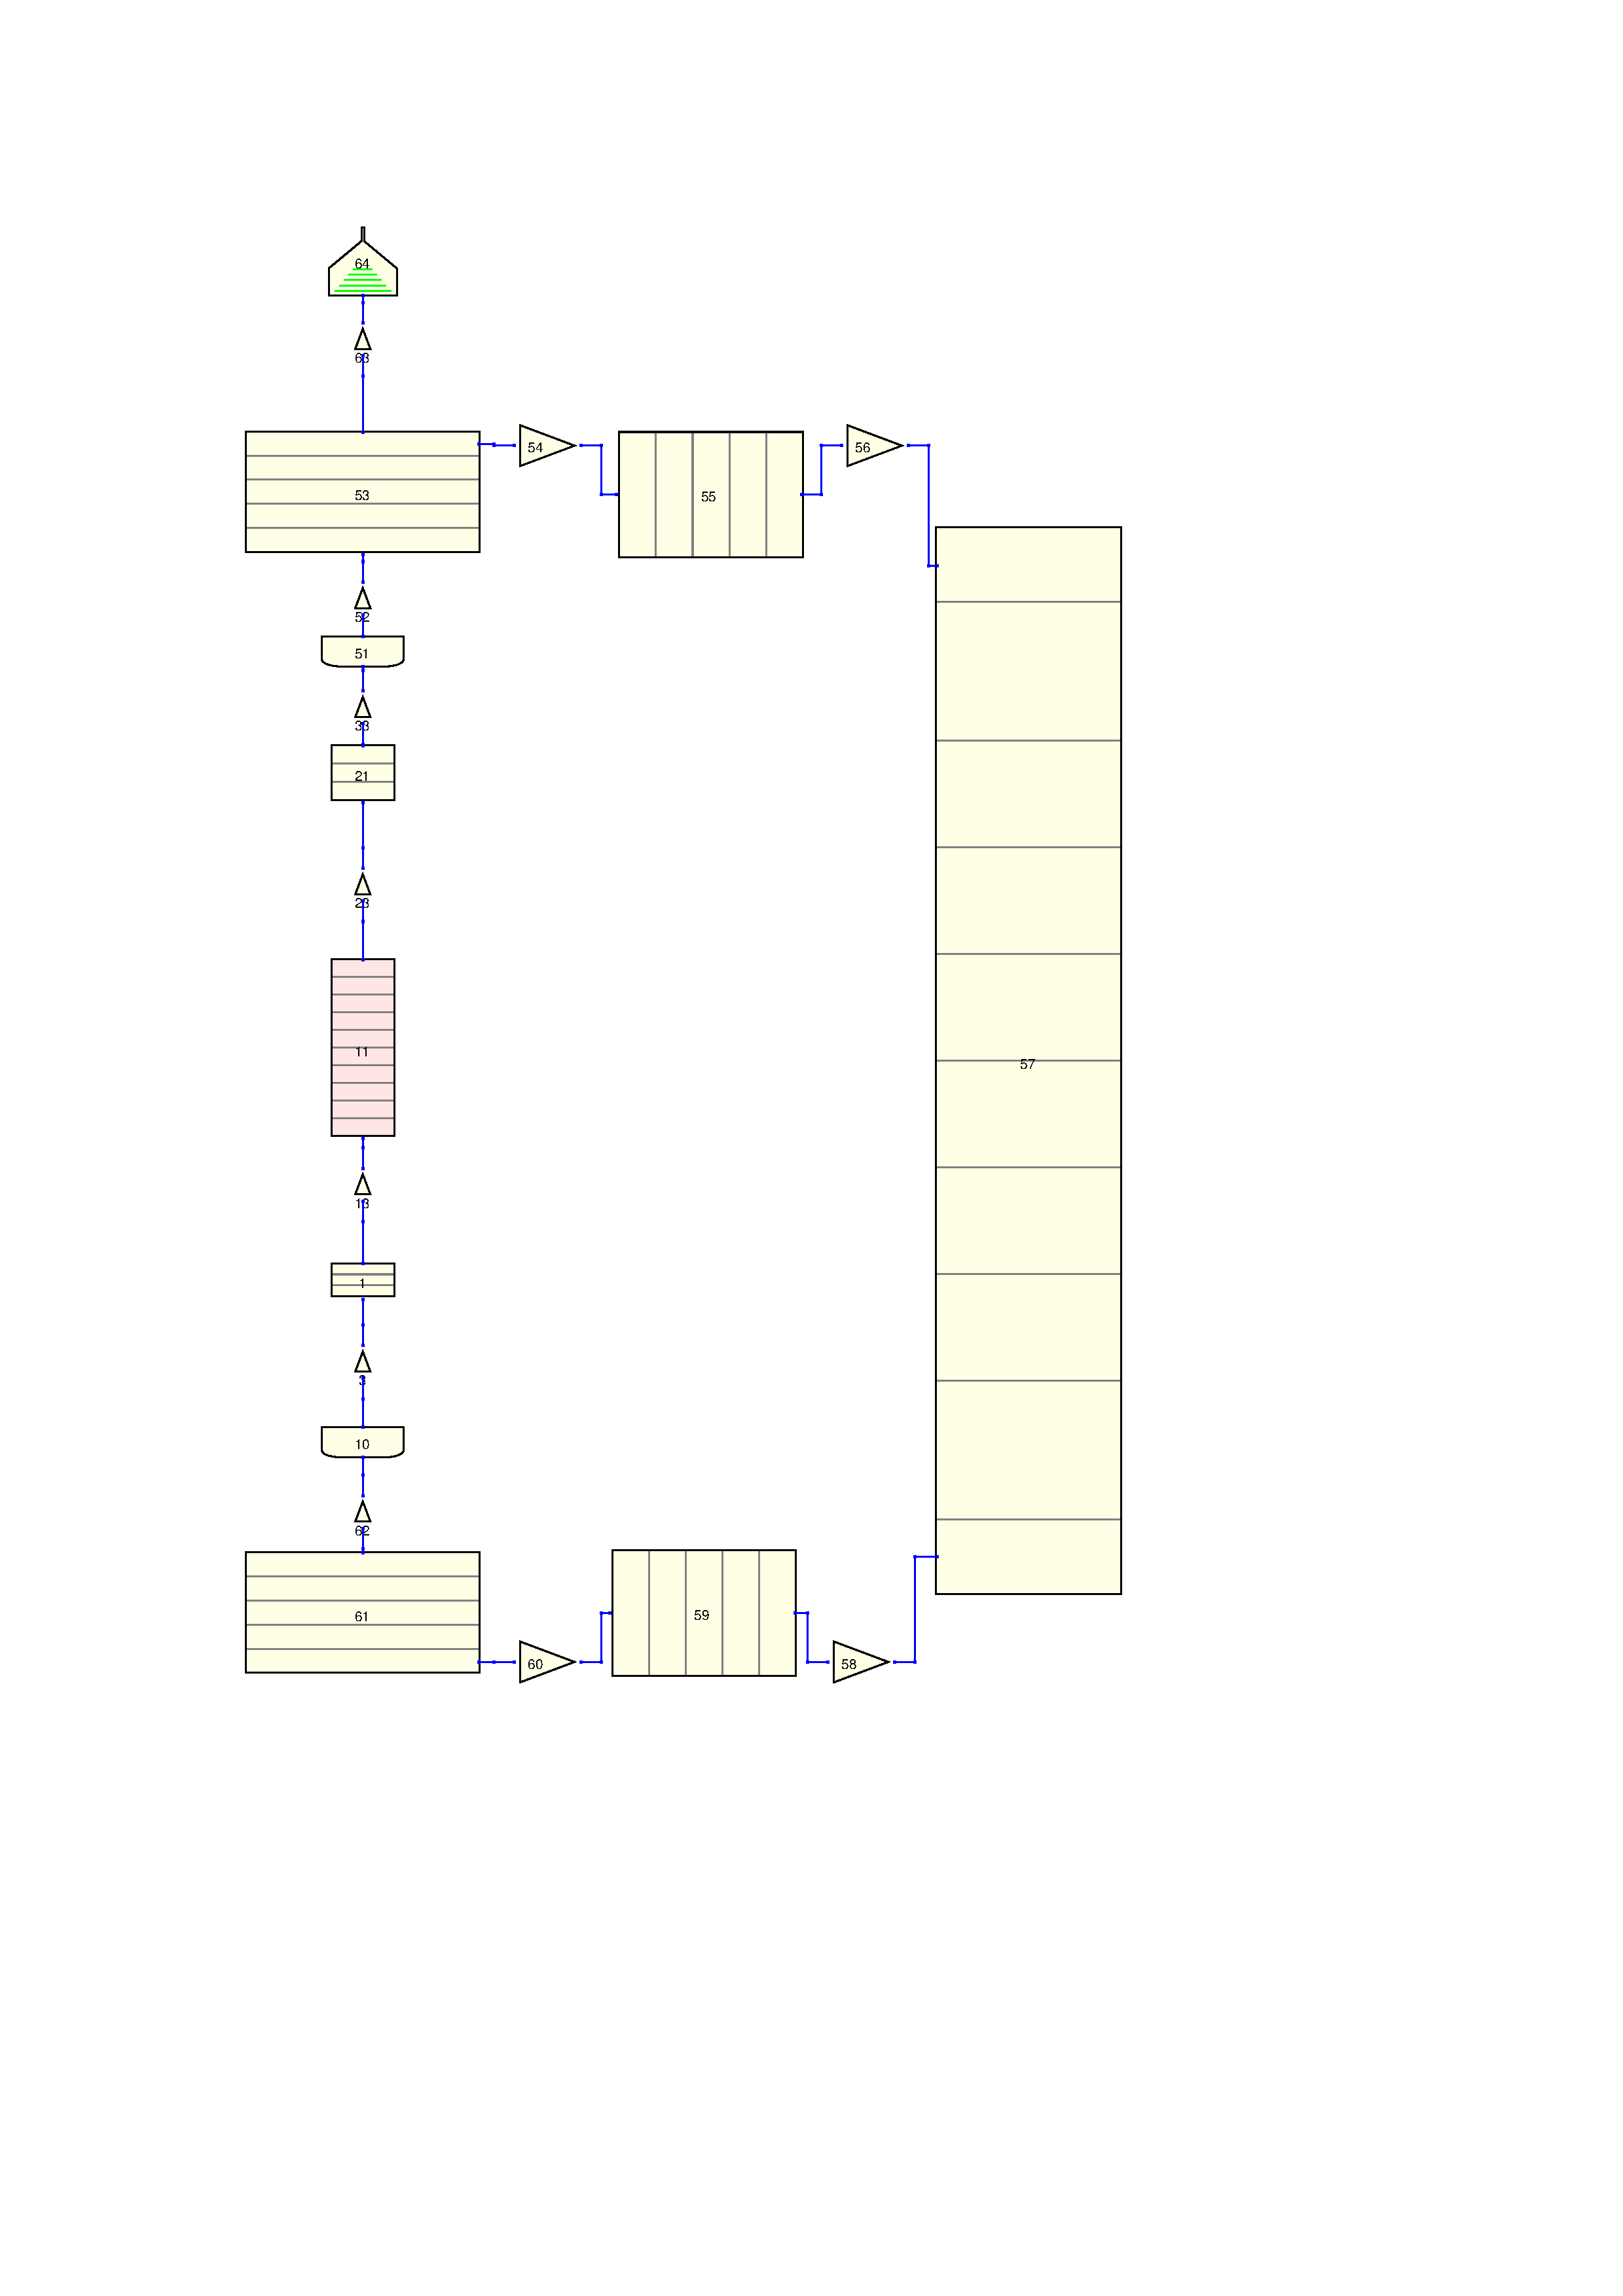
\includegraphics[width=\textwidth, trim={4cm 15cm 12cm 6cm}, clip]{./07_prilohy/prehled_modelu/t8bj.pdf}
	\caption{Termohydraulický zjednodušený model 8-trubkového PČ IRT-4M bez vytěsnitele (Pro lepší vizualizaci byly měřítka komponent 53-62 změněna).}
	\label{fig:irt_nat_conv_jedno}
\end{figure}

Pro vytvoření zdroje tepla v PČ byla uvažována dvě rozložení výkonu, a to rovnoměrné rozdělení a distribuce výkonu dle výpočetního programu Serpent2. V obou případech byl studován průtok, ohřev a výskyt povrchového bublinkového varu při přechodu z komplexního na zjednodušený model. Celkový výkon byl nastaven na 1,5$ \cdot 10^5$ W, přičemž pro rovnoměrné rozdělení se předpokládal zlomek výkonu v každém nódu 0.0125 (8 trubek, v každé 10 nódů), tedy každý nód produkuje 1875 W. Rozložení výkonu z programu Serpent2 je uvedeno v tab. \ref{tab:rozlozeni_vykonu_irt_serpent} a na Obr. \ref{fig:rozlozeni_vykonu_irt_serpent}.
\begin{table}[H]
	\centering
	\caption{Rozložení výkonu v 8-trubkovém PČ IRT-4M dle programu Serpent.}
	\label{tab:rozlozeni_vykonu_irt_serpent}
	\begin{tabular}{cc|cc}
		\hline
		Nód (-) & $P_{\text{rel}}^{\text{ax}}$ (-) & Palivová trubka & $P_{\text{rel}}^{\text{trubka}}$ (-) \\
		\hline \hline
		10 & 0,053 &  1& 0,22 \\
		9  & 0,081  & 2& 0,18 \\
		8  & 0,108  & 3& 0,15 \\
		7  & 0,126  & 4& 0,13 \\
		6  & 0,135  & 5& 0,11 \\
		5  & 0,135  & 6& 0,09 \\
		4  & 0,125  & 7& 0,08 \\
		3  & 0,106  & 8& 0,05 \\
		2  & 0,080  & &  \\
		1  & 0,052  & & \\
		\hline 
		
		
		
		
		
		
		
		
		
	\end{tabular} 
\end{table} 
\begin{figure}[H]
	\centering
	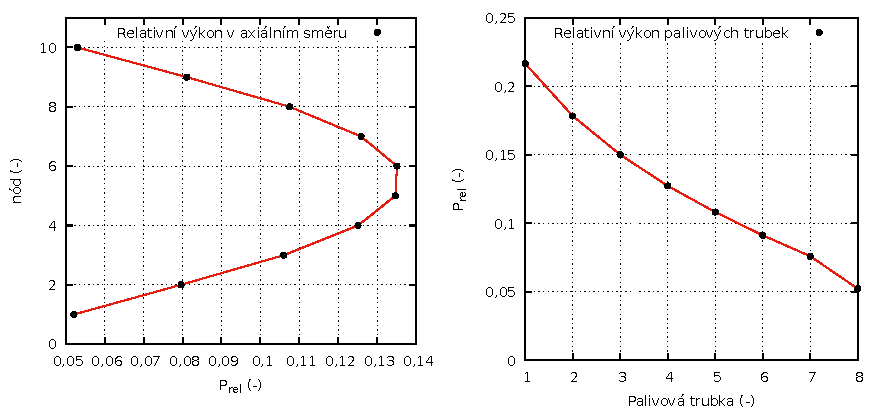
\includegraphics[width=0.8\textwidth]{./04_TH_model_IRT/grafy/average_power_distribution.pdf}
	\caption{Axiální a radiální rozložení výkonu v 8-trubkovém PČ IRT-4M - Serpent2.}
	\label{fig:rozlozeni_vykonu_irt_serpent}
\end{figure}
Axiální nodalizace palivových trubek v programu Serpent byla uvažována ve shodě s nodalizací trubek 21-29  viz Obr. \ref{fig:irt_nat_conv_komplex}, resp. trubky 11 viz Obr. \ref{fig:irt_nat_conv_jedno}. 

%V axiálním směru byla každá HS rozdělena na 10 nódů, přičemž zlomek celkového výkonu každé palivové trubky byl odlišný.  

\section{Sjednocení průtočných kanálů}
\label{sec:termohydraulicky_model_IRT}
Cílem následujícího textu je popsat problematiku sjednocení průtočných kanálů, porovnat výsledky komplexního a zjednodušeného modelu (viz Obr. \ref{fig:irt_nat_conv_komplex} a \ref{fig:irt_nat_conv_jedno}) pro dvě různé rozdělení výkonu a ověřit správnost zjednodušeného modelu. Sledovanými veličinami jsou celkový průtok skrz PČ (viz sekce \ref{subsec:nat_conv_prutok}), ohřev vody na výstupu z jednotlivých kanálů (viz sekce \ref{subsec:nat_conv_ohrev}) a možný výskyt povrchového bublinkového varu (viz sekce \ref{subsec:nat_conv_var}). 
\subsection{Celkový průtok skrz PČ}
\label{subsec:nat_conv_prutok}
Jak bylo výše odhadováno, tak při konjukci kanálů nedochází k zásadní změně v celkovém průtoku viz tab. \ref{tab:prutok_irt_nat_conv}. Vliv rozložení výkonu na průtok je možné považovat za bezvýznamný. 
\begin{table}[H]
	\centering
	\caption{Celkový průtok skrz PČ pro komplexní a zjednodušený model při rovnoměrném rozdělením výkonu a rozdělením dle programu Serpent2.}
	\label{tab:prutok_irt_nat_conv}
	\begin{tabular}{ll}
		\hline
		Rozložení výkonu \& Model & G (m$^3$/h) \\ \hline
		Rovnoměrný výkon - komplexní model      & 2,246 \\
		Serpent2 - komplexní model       & 2,247 \\
		Rovnoměrný výkon - zjednodušený model & 2,262 \\
		Serpent2 - zjednodušený model & 2,261 \\ \hline
	\end{tabular}
\end{table}
Z hlediska zachování celkového průtoku nevykazuje sjednocení kanálů výrazné rozdíly.

\subsection{Ohřev chladiva na výstupu z jednotlivých kanálů (trubek) PČ}
\label{subsec:nat_conv_ohrev}
Z Obr. \ref{fig:ohrev_kanal} a tab. \ref{tab:ohrev_irt_nat_conv} je vidět, že ohřev chladiva při rozdělení dle programu Serpent je značně rovnoměrnější, což jistě ovlivní i možný výskyt povrchového varu. Na Obr. \ref{fig:ohrev_kanal} je pro porovnání s komplexním modelem uveden ohřev na výstupu ze zjednodušeného modelu (jeden kanál). Maximální kanál v případě rovnoměrného rozdělení odpovídá trubce 27 (průtočná plocha 7 viz obr. \ref{fig:rad_irt_serpent}), což je stejný výsledek jako v \cite{fejt}. V případě rozdělení dle programu Serpent je maximální ohřev v trubce 22 (průtočná plocha 2 viz obr. \ref{fig:rad_irt_serpent}). Celkově ovšem výsledky korespondují s \cite{fejt}.

Z tab. \ref{tab:ohrev_irt_nat_conv} a Obr. \ref{fig:ohrev_vykon_rovn} a \ref{fig:ohrev_vykon_serpent} lze soudit, že nejtíživějším problémem při sjednocení trubek do zjednodušeného kanálu je právě ztráta informace o maximální teplotě ohřevu. Proti této ztrátě hraje fakt, že podíl rozdílu teplot v maximálním kanálu a zjednodušeném modelu zůstává pro naprostou většinu výkonů velice stálý. V obou případech rozložení výkonu se tento faktor pohybuje okolo hodnoty 1,13.  Vliv zjednodušení je více komentován v sekci \ref{subsec:nat_conv_zaver}.
\begin{figure}[H]
	\centering
	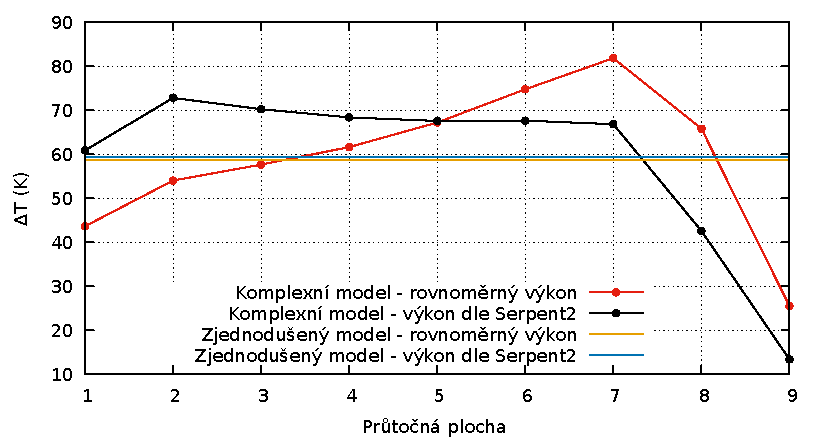
\includegraphics[width=\textwidth]{./04_TH_model_IRT/grafy/deltaT_irt4m_8_trubka.pdf}
	\caption{Ohřev na výstupu z jednotlivých kanálů pro jednotlivé modely.}
	\label{fig:ohrev_kanal}
\end{figure}
\begin{table}[H]
	\centering
	\caption{Ohřev chladiva na výstupu z PČ pro jednotlivé kanály (RV - rovnoměrný výkon, S - výkon dle Serpent2, KM \& JM - komplexní a zjednodušený model).}
	\label{tab:ohrev_irt_nat_conv}
	\begin{tabular}{llllllllll}
		\hline
		& \multicolumn{9}{c}{Trubka} \\ \hline
			$\Delta T_{out}$ (K) & 21 & 22 & 23 & 24 & 25 & 26 & 27 & 28 & 29          \\ \hline
		RV - KM   & 43,6     & 54,0    & 57,7    & 61,6    & 67,2    & 74,8    & 81,9    & 65,8    & 25,5    \\
		 S - KM     & 60,9    & 72,8    & 70,3    & 68,4    & 67,6    & 67,6    & 66,9    & 42,6    & 13,3     \\
		 RV - JM   & 58,7    &          &          &          &          &          &          &          &                         \\
		 S - JM & 59,3    &          &          &          &          &          &          &          &          \\         \hline      
	\end{tabular}
\end{table}

\begin{figure}[H]
	\centering
	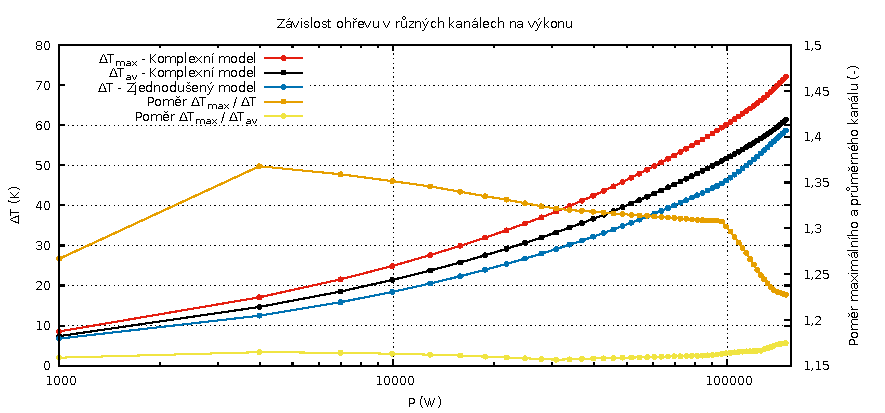
\includegraphics[width=\textwidth]{./04_TH_model_IRT/grafy/ohrev_rovn.pdf}
	\caption{Závislost ohřevu pro komplexní a zjednodušený model - rovnoměrný výkon (poměr teplot je poměr rozídlu teploty na výstupu z kanálu zjednodušeného modelu a komplexního modelu).}
	\label{fig:ohrev_vykon_rovn}
\end{figure}
\begin{figure}[H]
	\centering
	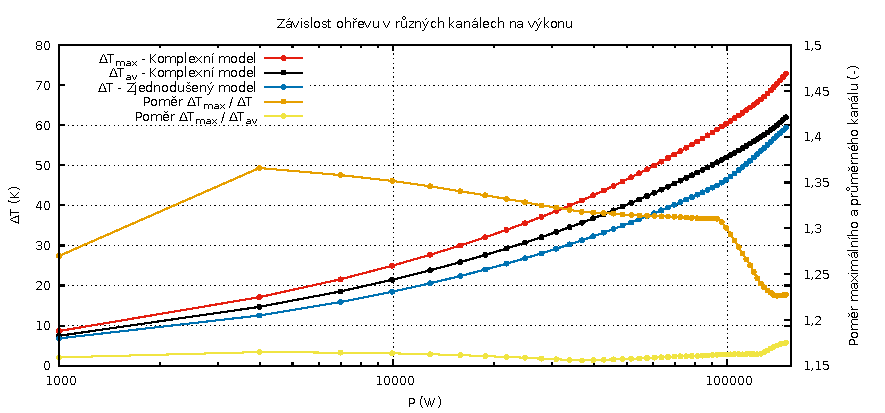
\includegraphics[width=\textwidth]{./04_TH_model_IRT/grafy/ohrev_serpent.pdf}
	\caption{Závislost ohřevu pro komplexní a zjednodušený model - výkon dle Serpent2 (poměr teplot je poměr rozídlu teploty na výstupu z kanálu zjednodušeného modelu a komplexního modelu).}
	\label{fig:ohrev_vykon_serpent}
\end{figure}

\subsection{Výskyt povrchového varu}
\label{subsec:nat_conv_var}
Možný výskyt varu v této sekci představuje stav, kdy teplota HS je vyšší než teplota sytosti kapaliny. Výkon jedné HS představující trubku PČ je \SI{1,875e4}{\watt}, tedy celkový výkon PČ je \SI{1,5e5}{\watt}.
Jak již bylo avizováno, tak při rozdělení výkonu dle programu Serpent je rozdělení teplot daleko rovnoměrnější, cž vede i k rovnoměrnějšímu výskytu možného povrchového bublinkového varu. Zároveň lze ale pozorovat, že konjukce trubek nemá na možný výskyt povrchového varu vliv.
\begin{figure}[H]
	\centering
	\begin{minipage}{.5\textwidth}
		\centering
		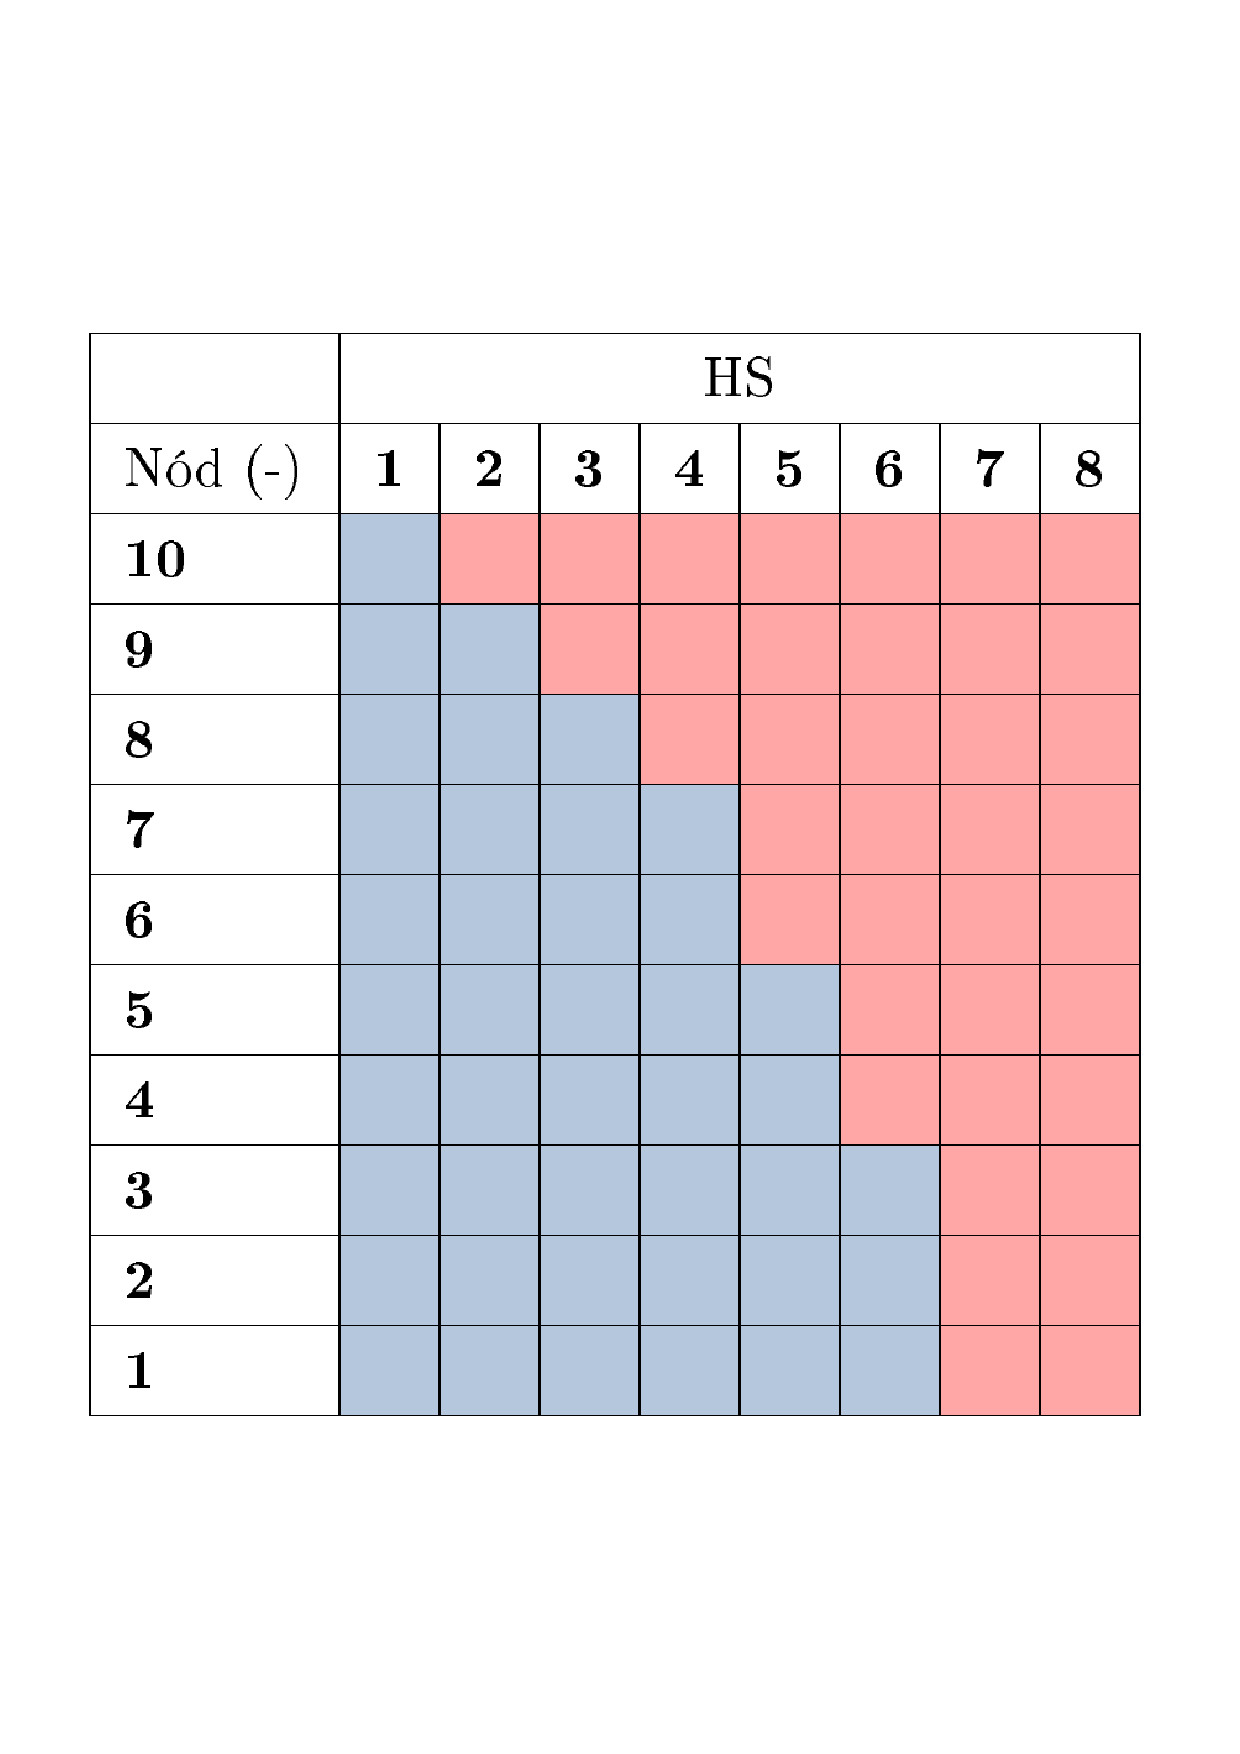
\includegraphics[width=0.98\textwidth, trim={1cm 5.5cm 0.5cm 5.5cm}, clip]{./04_TH_model_IRT/grafy/var_rovn_komplex.pdf}
		\caption{Komplexní model}
		\label{fig:var_komplex_rovn}
	\end{minipage}%
	\begin{minipage}{.5\textwidth}
		\centering
		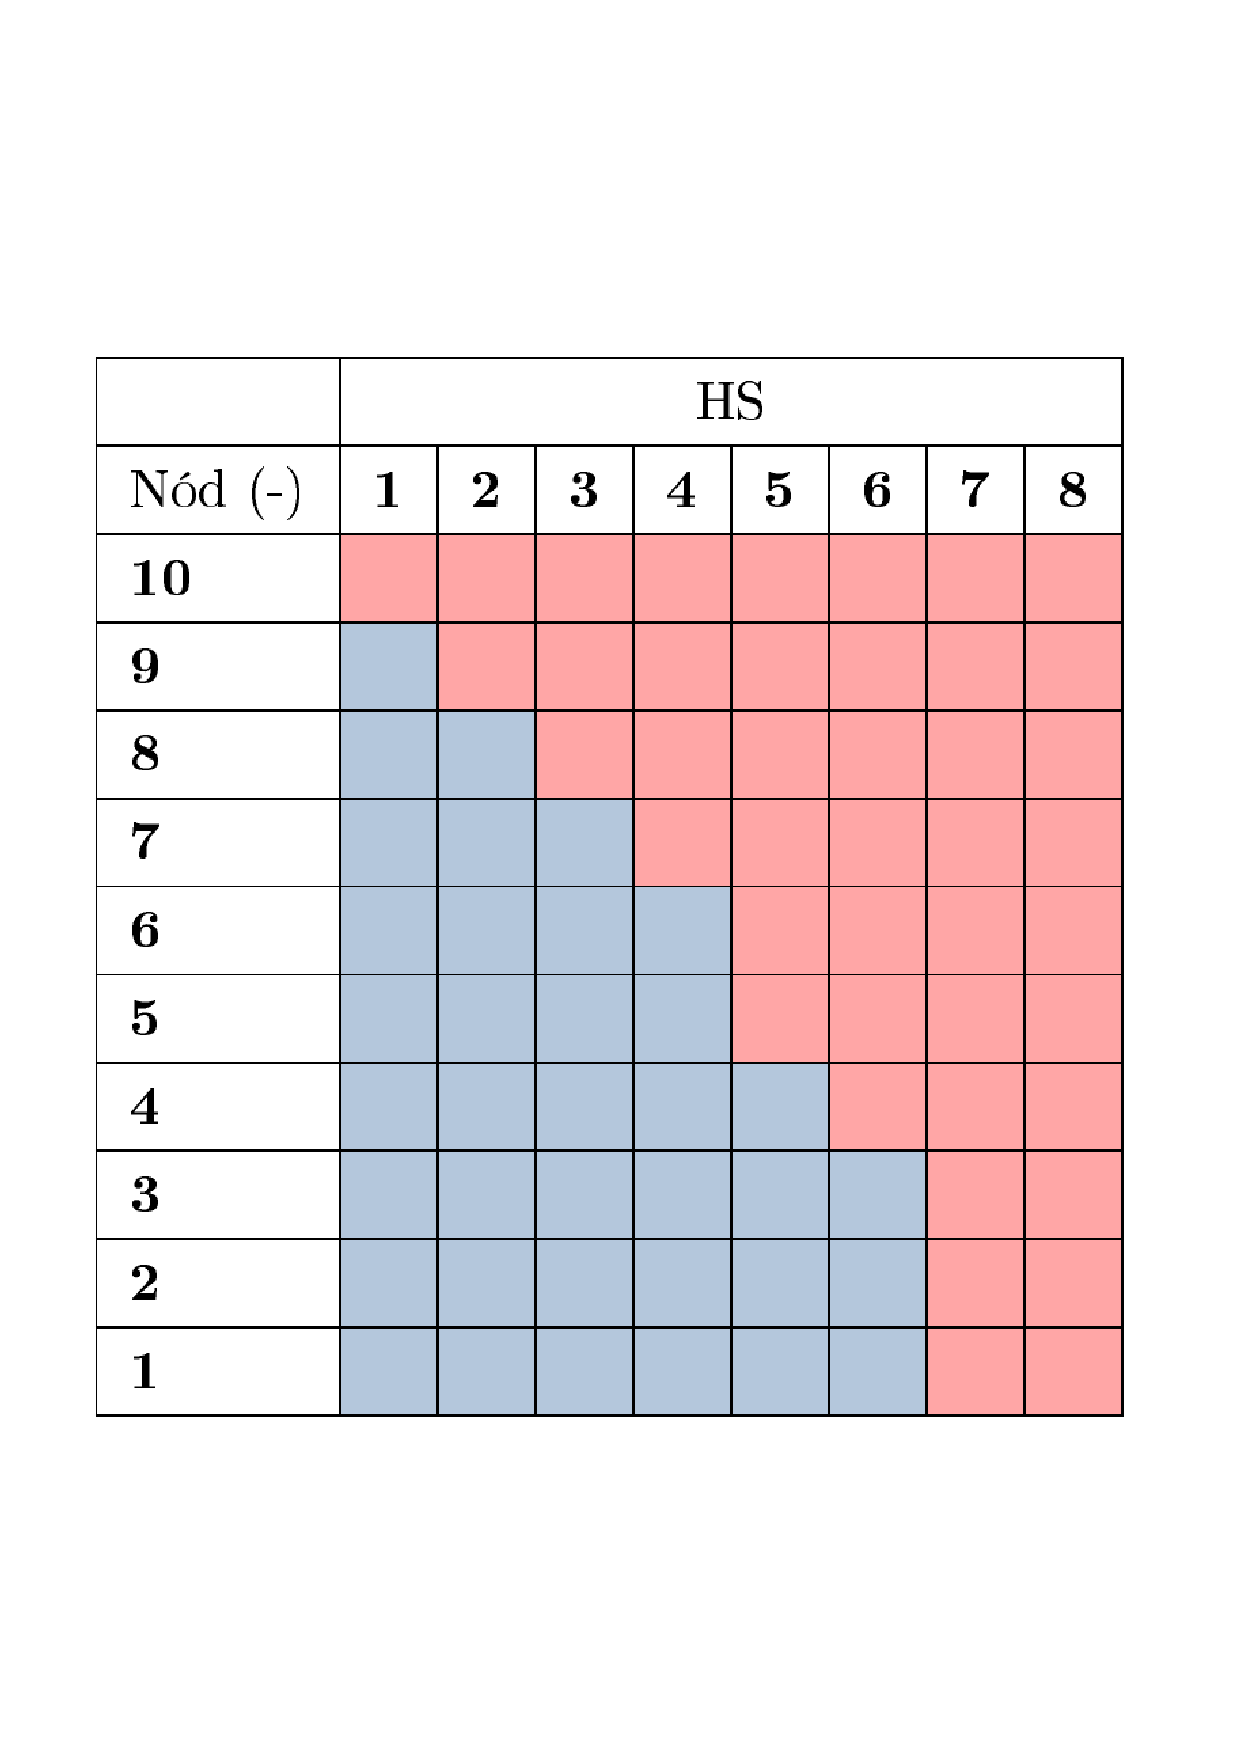
\includegraphics[width=\textwidth, trim={1cm 5.5cm 0.5cm 6cm}, clip]{./04_TH_model_IRT/grafy/var_rovn_jedno.pdf}
		\caption{Zjednodušený model}
		\label{fig:var_jedno_rovn}
	\end{minipage}
\caption{Možný výskyt povrchového bublinkového varu - rovnoměrné rozdělení výkonu (červeně nódy označují možný výskyt varu, modré přirozenou konvekci bez změny fáze).}
\label{fig:var_rovn}
\end{figure}
\begin{figure}[H]
	\centering
	\begin{minipage}{.5\textwidth}
		\centering
		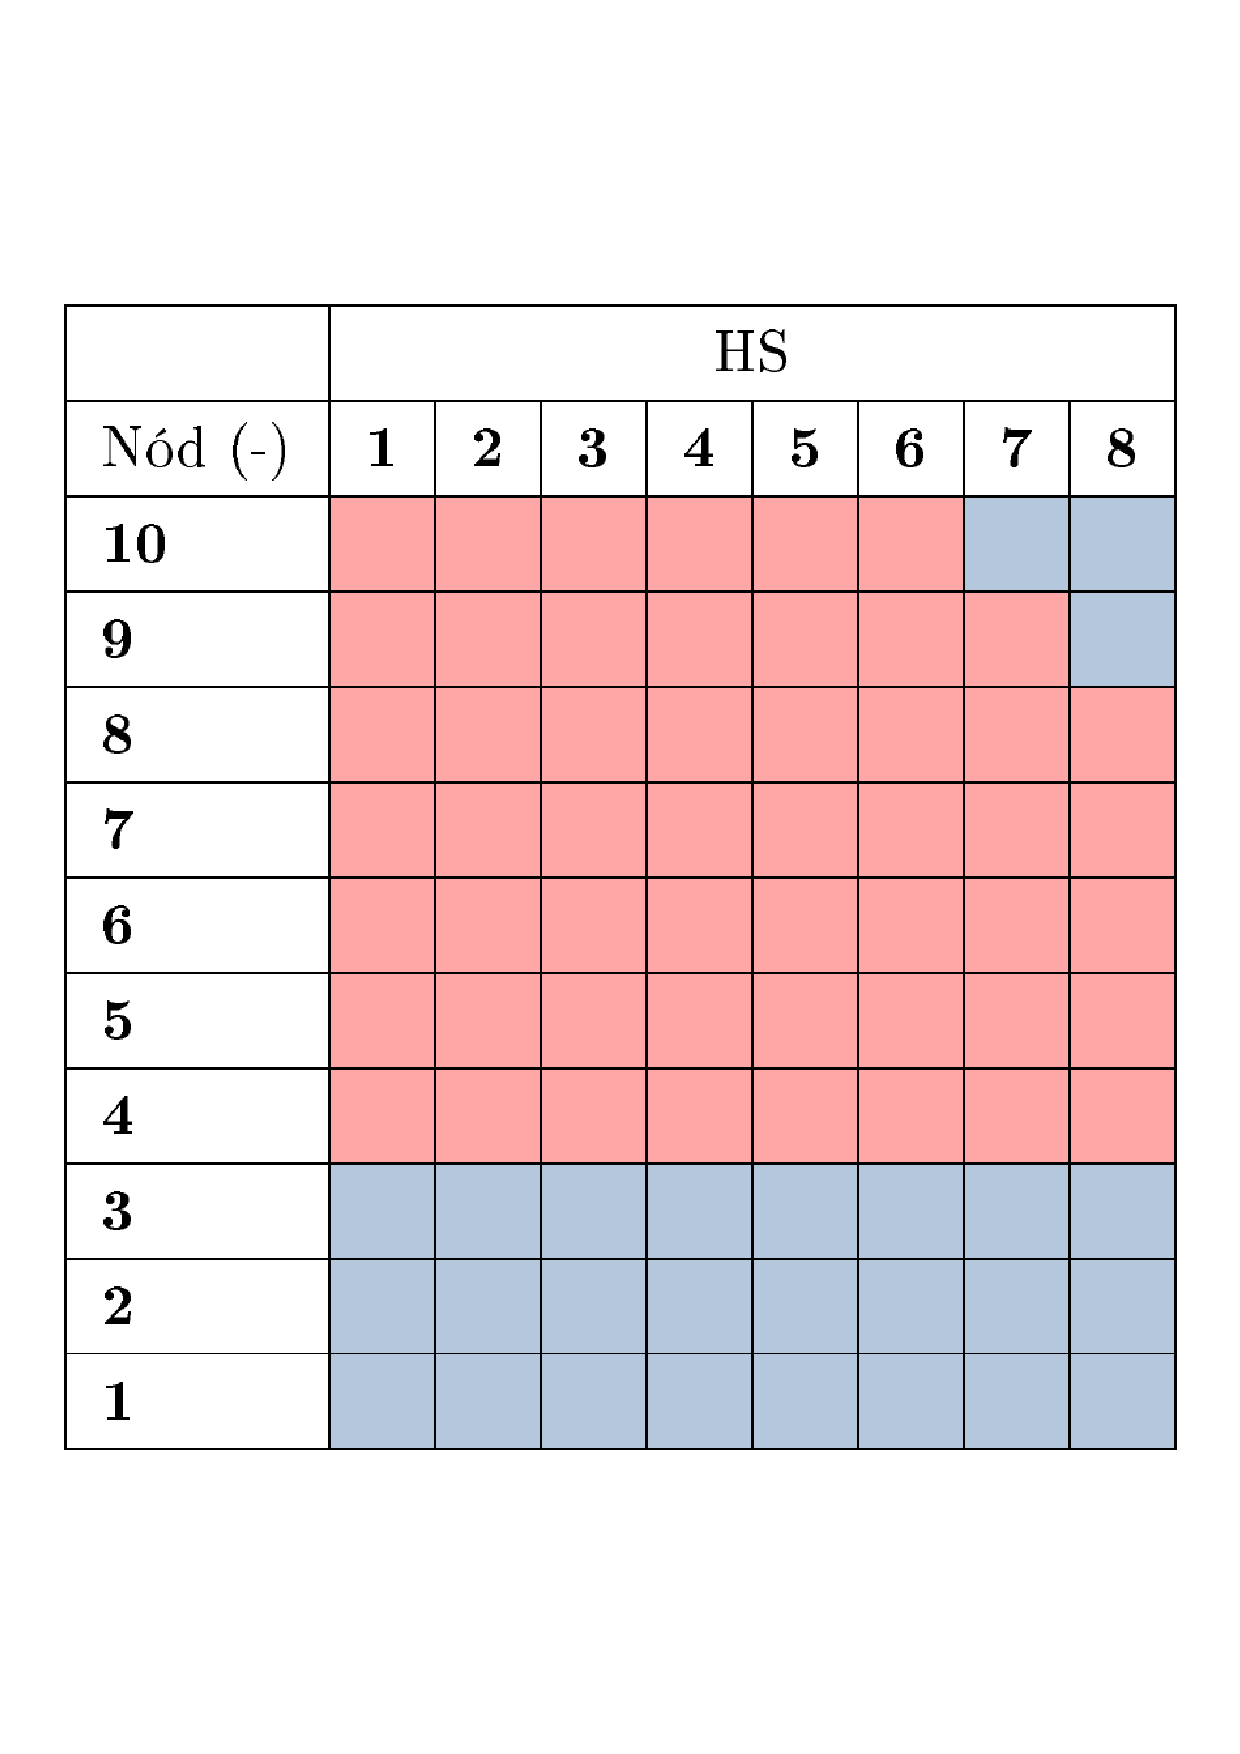
\includegraphics[width=0.98\textwidth, trim={0.5cm 4cm 0cm 5cm}, clip]{./04_TH_model_IRT/grafy/var_serpent_komplex.pdf}
		\caption{Komplexní model}
		\label{fig:var_komplex_serpent}
	\end{minipage}%
	\begin{minipage}{.5\textwidth}
		\centering
		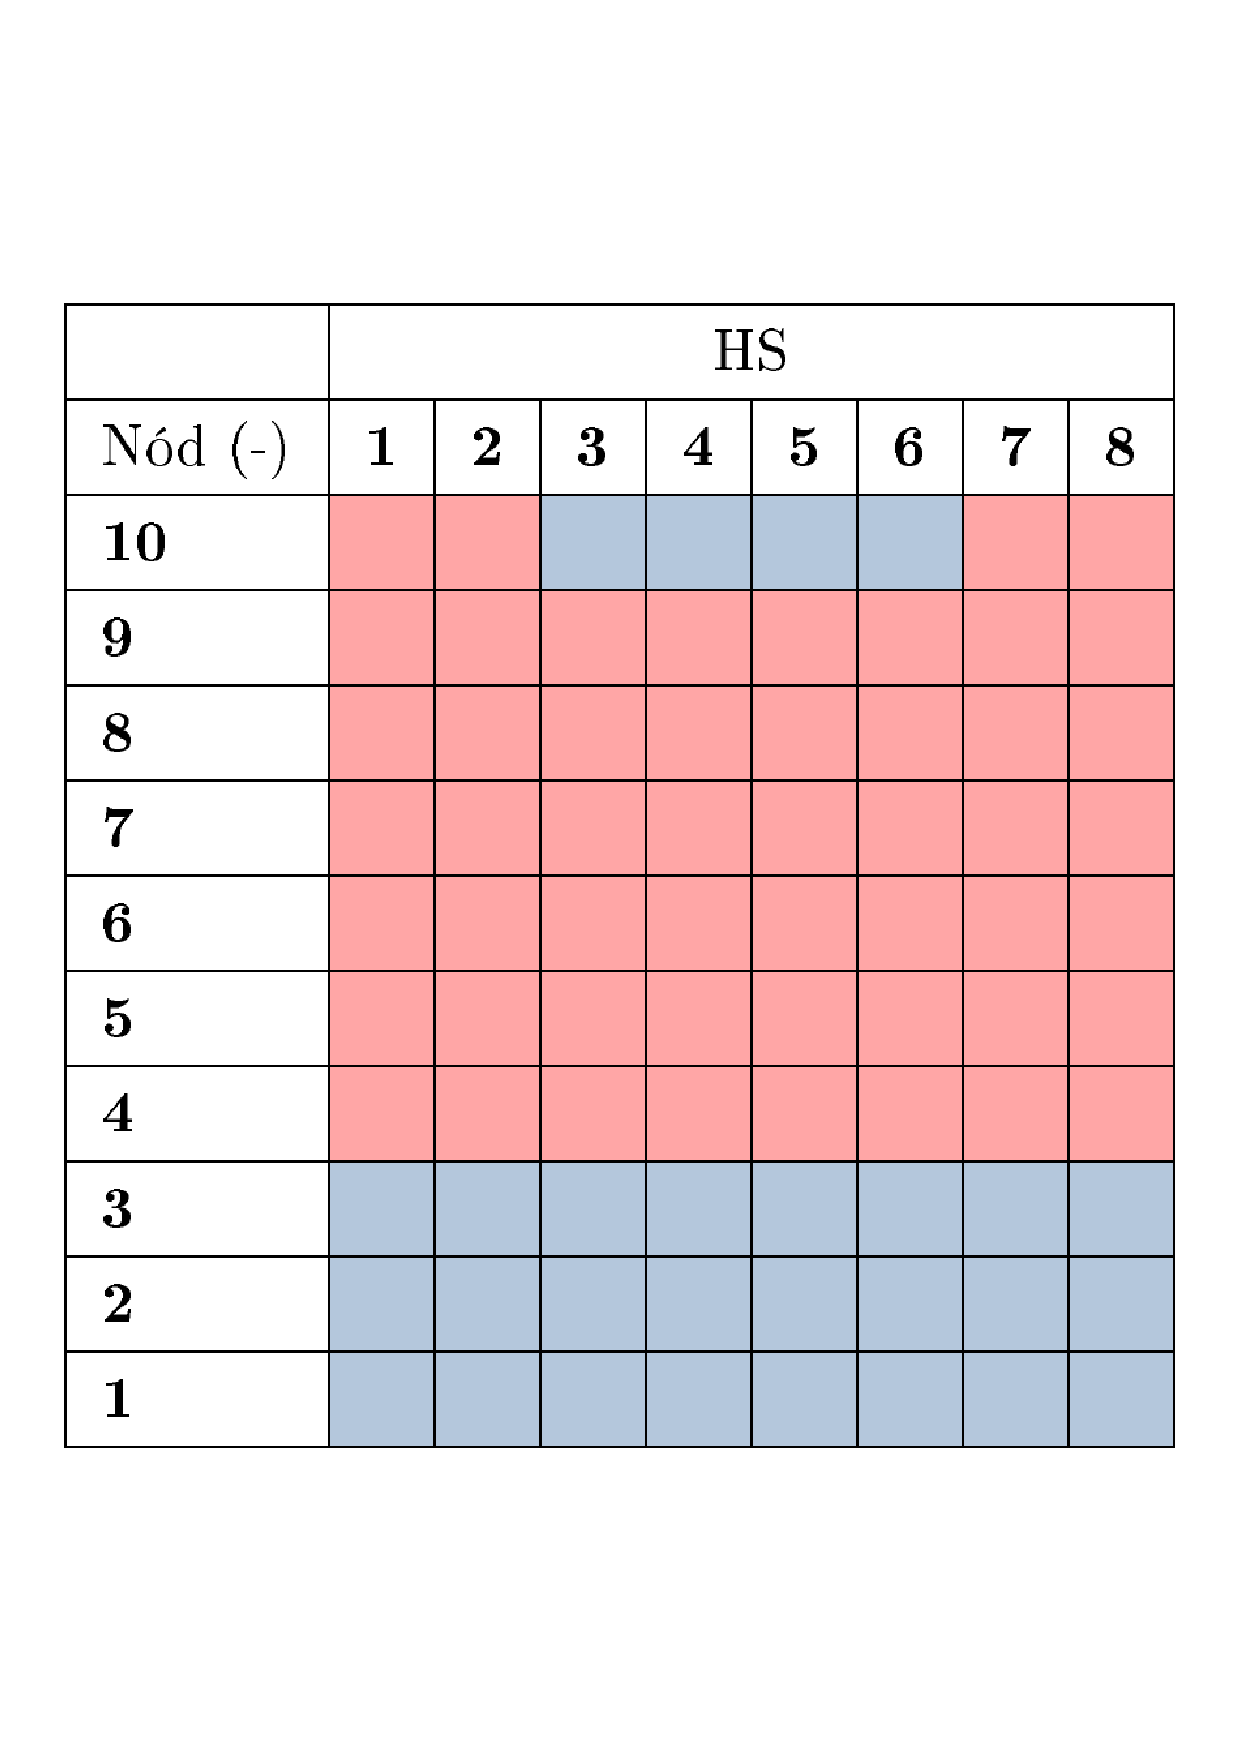
\includegraphics[width=0.98\textwidth, trim={0.5cm 4cm 0cm 5cm}, clip]{./04_TH_model_IRT/grafy/var_serpent_jedno.pdf}
		\caption{Zjednodušený model}
		\label{fig:var_jedno_serpent}
	\end{minipage}
	\caption{Možný výskyt povrchového bublinkového varu - rozdělení výkonu dle Serpent2 (červeně nódy označují možný výskyt varu, modré přirozenou konvekci bez změny fáze).}
	\label{fig:var_serpent}
\end{figure}
\subsection{Zhodnocení sjednocení průtočných kanálů}
\label{subsec:nat_conv_zaver}
Sjednocení průtočných kanálů nenaznačují žádný velký problém pro další použití. Největším problémem je právě ztráta informace o maximálním ohřevu, což může být do jisté kompenzováno již zmiňovaným \uv{faktorem ohřevu}. Ukazuje se, že tento faktor zůstává konstantní pro široké rozmezí výkonů a je možné tedy provést odhad maximální teploty na výstupu z PČ. Dále se ukazuje, že rozložení výkonu způsobuje rovnoměrnější ohřev a možný výskyt povrchového bublinkového varu. Sjednocení na možný povrchový var nemá velký vliv. Největším problémem pro bezpečnostní analýzy by v tomto případě byla situace, kdy by v maximálním kanálu docházelo k objemovému varu. Vznik objemového varu ovšem není součástí základních projektových podmínek ani rozšířených projektových podmínek \cite{fejt, rataj_bezpecnosti_zprava_VR_1}.



\section{Sjednocení topných komponent} \label{sec:sjednoceni_topnych_komponent}
Pro analýzu přirozeného proudění skrz PČ IRT-4M dává smysl využít počet HS odpovídající počtu palivových trubek, tedy 8 topných jednotek. Pro analýzu celé aktivní zóny reaktoru VR-1 by bylo třeba vložit okolo 8$\times$16 HS, což by mohlo být problematické. Proto dává smysl vytvořit zjednodušený model se sjednocenými topnými komponentami. Při přechodu na jednu zjednodušenou HS je třeba zachovat stejnou teplosměnnou plochu a hydraulický průměr. V tab. \ref{tab:jednotkovy_model} geometrie této HS uvedena. Vnější průměr sjednocené HS v tomto případě převyšuje vnější rozměr palivové trubky 1 viz tab. \ref{tab:prilohy_irt_geometrie}, což je konstruktem požadavku na zachování teplosměnné plochy a hydraulického průměru. Tato HS chováním reprezentuje komplexní sadu 8 HS a je dále využitá jakožto zdroj tepla pro PČ v termohydraulickém modelu VR-1. Zjednodušený model PČ s sjednocenou HS bude dále označován jako \uv{jednotkový model}. Rozdíl zjednodušeného a jednotkového modelu je pouze v HS, geometrie trubek a obtoku zůstává stejná. Axiální rozložení výkonu odpovídá tab. \ref{tab:rozlozeni_vykonu_irt_serpent} uvedené v předchozí sekci.
\begin{table}[H]
	\centering
	\caption{Geometrie sjednocené HS.}
	\label{tab:jednotkovy_model}
	\begin{tabular}{cc}
		\hline
		$ r_o $ (mm) & 210,11  \\
		$ r_i $ (mm) & 207,82  \\
		$ h $ (mm) 	 & 588 \\
		
		\hline
	\end{tabular}
\end{table}
\subsection{Výpočet a zhodnocení sjednocení HS}
Analogicky k předchozí části jsou v tab. \ref{tab:sjednoceni_hs} uvedeny parametry pro zjednodušený model (1 průtočná trubka a 8 HS) a jednotkový model (1 průtočná trubka a 1 sjednocená HS). Namísto možného výskytu povrchového varu je v tabulce uvedena maximální teplota HS.
\begin{table}[H]
	\centering
	\caption{Celkový průtok, ohřev a maximální teplota HS pro zjednodušený a jednotkový model.}
	\label{tab:sjednoceni_hs}
	\begin{tabular}{cccc}
		\hline
		& \multicolumn{2}{l}{TH model}          &                    \\
		& zjednodušený (serpent) & jednotkový   & rel. odch. (\%)    \\
		\hline \hline

		$G$ (m$^3$/h) & 2,261 & 2,258 & 0,11\\
		$\Delta T$ (K)                & 59,31                  & 59,38        & 0,12 \\
		$T_{\text{HS},\text{max}}$ (K)             & 384,85                 & 383,54       & 0,34\\
		\hline
	\end{tabular}
\end{table}
 Změna v průtoku chladiva skrz PČ a změna ohřevu je zanedbatelná, maximální teplota HS se liší o méně než 0,5 \%. Z uvedených výsledků vyplývá, že je možné považovat jednotkový model za způsobilý dalším výpočtům. Oproti zjednodušenému modelu je výhodou redukovaný počet HS, který by při složitějších výpočtech AZ mohl být komplikovaný.